% ============================================================
% Cascade Impingement Swirl Tray (CIST)
% HyTray Invention Disclosure Series
% ============================================================
\documentclass[11pt,letterpaper]{article}

% ── packages ─────────────────────────────────────────────────────────────────
\usepackage[top=1.0in, bottom=1.0in, left=1.0in, right=1.0in]{geometry}
\usepackage{amsmath,amssymb}
\usepackage{booktabs}
\usepackage{graphicx}
\usepackage[colorlinks=true,linkcolor=blue!60!black,citecolor=blue!60!black,
            urlcolor=blue!60!black]{hyperref}
\usepackage{siunitx}
\DeclareSIUnit\inch{in.}
\DeclareSIUnit\psi{psi}
\usepackage{tabularx}
\usepackage{longtable}
\usepackage{caption}
\usepackage{subcaption}
\usepackage{fancyhdr}
\usepackage{enumitem}
\usepackage{array}
\usepackage{multirow}
\usepackage{float}
\usepackage[expansion=false]{microtype}
\usepackage{parskip}
\usepackage{xcolor}
\usepackage{mathtools}

% ── page style ───────────────────────────────────────────────────────────────
\pagestyle{fancy}
\fancyhf{}
\rhead{\small HyTray Invention Disclosure Series}
\lhead{\small Cascade Impingement Swirl Tray (CIST)}
\cfoot{\small\thepage}
\renewcommand{\headrulewidth}{0.4pt}

% ── math short-hands ─────────────────────────────────────────────────────────
\newcommand{\rhoL}{\rho_L}
\newcommand{\rhoV}{\rho_V}
\newcommand{\ujet}{u_{\mathrm{jet}}}
\newcommand{\utheta}{u_{\theta}}
\newcommand{\ux}{u_{x}}
\newcommand{\Ntu}{N_{\mathrm{OG}}}
\newcommand{\Eog}{E_{\mathrm{OG}}}
\newcommand{\dpc}{\Delta P_c}
\newcommand{\dptot}{\Delta P_{\mathrm{total}}}
\newcommand{\Rc}{R_c}
\newcommand{\Hc}{H_c}
\newcommand{\Dc}{D_c}
\newcommand{\dsv}{d_{32}}
\newcommand{\dmin}{d_{\min}}
\newcommand{\dcut}{d_{50}}
\newcommand{\Lsw}{L_{\mathrm{AS}}}
\newcommand{\We}{\mathit{We}}
\newcommand{\Stk}{\mathit{Stk}}
\newcommand{\Rey}{\mathit{Re}}
\newcommand{\Csb}{C_{\mathrm{SB}}}
\newcommand{\Hcol}{H_{\mathrm{col}}}

% ── caption formatting ────────────────────────────────────────────────────────
\captionsetup{font=small,labelfont=bf}

% ════════════════════════════════════════════════════════════════════════════
\begin{document}

% ── title block ──────────────────────────────────────────────────────────────
\begin{center}
  {\large\bfseries HyTray Invention Disclosure Series}\\[4pt]
  {\LARGE\bfseries Cascade Impingement Swirl Tray (CIST):\\
  A Jet-Fed Swirl-Chamber Distillation Stage\\
  with Elliptical Liquid Nozzles}\\[8pt]
  {\large A distillation tray in which vapour--liquid contact occurs
  in a free swirl-shear zone between opposing jet streams,\\
  decoupled from the gravity-settling flooding limit of conventional decks}\\[10pt]
  \textit{Inventor:} Pratik\\[4pt]
  \textit{Invention Disclosure / Provisional Specification Draft --- HyTray Series HT-CI}\\
  June 2026
\end{center}

\hrule\vspace{6pt}

% ── abstract ─────────────────────────────────────────────────────────────────
\begin{abstract}
\noindent
A distillation-column tray is disclosed in which vapour--liquid contacting
takes place inside an array of short cylindrical swirl chambers, each fed
independently by two fluid streams: (i) a liquid jet directed upward
through a calibrated elliptical orifice in the chamber floor, powered
solely by the liquid static head in the below-tray sump, and (ii) vapour
admitted tangentially through a slot in the lower chamber wall, generating
a rotating flow field.  There is no liquid pool on the tray deck and no
perforated flat plate.  The swirling vapour shears the ascending liquid
jet into a fine annular film and droplet cloud; the rotating two-phase
dispersion contacts across the full chamber volume.  A fixed-vane crown
separator at the chamber top separates the phases centrifugally, passing
clean vapour upward and discharging separated liquid outward into a
collection ring that drains by sealed conduit to the sump of the next tray
below.  The elliptical nozzle geometry (aspect ratio $k = a/b = 1.5$--2.5)
exploits the axis-switching instability of non-circular jets to produce
finer, more uniform droplets than a circular nozzle of equal flow area,
increasing interfacial area in the contact zone.  The capacity flooding
limit is set by centrifugal re-entrainment in the crown, not by gravity
settling, predicting a column-diameter reduction of the order of 35--45\%
relative to a conventional sieve tray at equal tray spacing.  Predicted
tray efficiency (90\% one-pass point efficiency at design conditions) and
turndown (6:1 to 8:1, limited by minimum swirl coherence) are estimated
from penetration-theory and Stokes-flow models respectively.  All
performance values are model predictions; they require cold-flow and
hot-rig validation before use in detailed design.
\end{abstract}

\noindent\textit{Status:} All equations and performance estimates in this
disclosure are derived from first-principles fluid mechanics and mass-transfer
correlations applied to an idealised geometry.  No prior tray performance
database has been used to calibrate the model.  The physical sub-models
(Rayleigh--Plateau jet instability, Rankine vortex, Stokes centrifugal
collection, penetration-theory mass transfer) are each individually
well-established; their application to this combined configuration, and
particularly the assumed design parameters (centripetal acceleration, nozzle
discharge coefficient, crown collection efficiency), requires experimental
confirmation.

\hrule\vspace{6pt}

\tableofcontents
\newpage

% ════════════════════════════════════════════════════════════════════════════
\section{Field of the Invention}

Vapour--liquid contacting internals for distillation, absorption and
stripping columns, specifically a tray-type stage in which vapour--liquid
contact is achieved by opposed jet impingement and swirl-shear mixing inside
enclosed cylindrical chambers, eliminating the gravity-dependent liquid pool
and perforated-plate deck of conventional tray designs.

% ════════════════════════════════════════════════════════════════════════════
\section{Background and Prior Art}

Every conventional distillation tray --- whether sieve, valve, or corrugated
--- shares a common operating principle: vapour passes upward through
perforations or valve openings in a horizontal deck, bubbling through a
shallow liquid pool maintained by an outlet weir.  The vapour--liquid
dispersion (froth) on the deck is the contact zone.  Phase separation after
contact occurs by gravity: liquid drains over the weir to the tray below,
and vapour rises clear of the froth.

This configuration imposes three capacity limitations that have not been
eliminated simultaneously by any commercial design:

\begin{enumerate}[nosep]
  \item \textbf{Gravity-settling entrainment limit (Souders-Brown criterion).}
    Above a critical vapour velocity $u_{\mathrm{SB}}$, liquid droplets
    entrained from the froth surface cannot settle against the rising vapour
    stream.  This limit depends on tray spacing and system properties but not
    on any tray geometry parameter under the designer's control beyond the
    tray-to-tray height.

  \item \textbf{Liquid weep limit.}
    Below a minimum vapour velocity, the upward kinetic pressure of the vapour
    is insufficient to support the liquid head above the perforations and
    liquid ``weeps'' downward through the holes, bypassing contact on the
    tray above.  This sets the lower end of the operating range and limits
    turndown to roughly 2:1--3:1 for conventional sieve and fixed-valve decks.

  \item \textbf{Downcomer-backup limit.}
    Liquid from the active deck must descend to the tray below through
    downcomers, which require a fraction (typically 15--25\%) of the column
    cross-section for their area.  At high liquid rates, the downcomer backup
    can reach the tray above, flooding the column independently of the vapour
    rate.
\end{enumerate}

Spray-tray and jet-tray concepts have partially addressed the entrainment
limit by using mechanical energy (liquid spray) for contact rather than
froth aeration, but they typically produce low tray efficiency (short droplet
residence time, no multi-pass liquid path) and poor turndown (spray quality
collapses at low liquid rate).  Centrifugal contactors
(cyclone trays, swirl-tube stages) have addressed the entrainment limit by
substituting centrifugal for gravitational phase separation, but known
designs retain a liquid pool on the deck as the liquid feed to each
contactor, re-introducing both the weep limit and the deck-pool entrainment
behaviour at the deck surface between contactors.

The CIST eliminates the deck pool entirely.  Liquid is fed to each chamber
as a coherent jet from below, metered by nozzle hydraulics rather than a weir
and pool.  Vapour is fed tangentially into the chamber rather than axially
through a perforation.  Both the contact zone and the phase-separation zone
are inside the chamber, making the tray-level flooding limit a function of
the swirl field strength, not gravity.

% ════════════════════════════════════════════════════════════════════════════
\section{Objects of the Invention}

\begin{enumerate}[nosep]
  \item To eliminate the deck liquid pool, replacing it with a controlled
    liquid jet fed from a below-tray sump, removing the weep-driven minimum
    vapour-rate constraint of perforated-plate decks.

  \item To replace gravity-settling phase separation with centrifugal
    separation inside each contact chamber, raising the effective capacity
    factor by a factor of the order of $\sqrt{N_g}$, where $N_g = a_c/g$
    is the centrifugal gravity ratio.

  \item To use elliptical rather than circular liquid-jet nozzles to exploit
    axis-switching jet instability, producing finer and more uniform droplets
    at the same volumetric flow rate, thereby increasing interfacial area per
    unit chamber volume.

  \item To achieve tray efficiency above 80\% one-pass point efficiency by
    ensuring that the swirling vapour--liquid dispersion contacts across the
    full chamber height before phase separation at the crown.

  \item To provide a stable operating range of at least 6:1 turndown from
    the lower limit (set by minimum swirl for centrifugal separation) to the
    upper limit (set by crown re-entrainment).

  \item To reduce tray pressure drop relative to conventional decks by
    eliminating the aerated-liquid-pool contribution $\beta h_{\mathrm{cl}}$
    to the pressure balance, replacing it with a smaller vapour-momentum
    loss through the swirl chamber.

  \item To provide a fully cartridge-maintainable stage: all swirl chambers
    and nozzle assemblies removable through the column manway without shell
    welding, and all wetted surfaces accessible for inspection.
\end{enumerate}

% ════════════════════════════════════════════════════════════════════════════
\section{Summary of the Invention}

The CIST deck (Figure~\ref{fig:elevation}) comprises a horizontal inter-tray
plate carrying an array of cylindrical contact chambers on a triangular
pitch, a below-plate sump that collects descending liquid, and a liquid
overflow seal (weir leg) to the sump of the tray below.

Each contact chamber is a vertical cylinder of inside diameter $\Dc$ and
height $\Hc = (1.2$--$2.0)\Dc$.  An elliptical orifice (nozzle) is machined
in the chamber floor; liquid in the sump drives a coherent upward jet through
this nozzle under the sump's hydrostatic head.  A tangential vapour inlet
slot in the lower chamber wall directs the vapour stream circumferentially,
establishing a Rankine-type vortex.  The ascending liquid jet is sheared by
the rotating vapour into an annular film on the chamber wall and a central
droplet cloud.  Mass transfer proceeds across both the film and the droplet
surfaces as the two-phase dispersion ascends the chamber.  A vane crown at
the chamber top intercepts the dispersion: the heavier liquid phase is
deflected outward by centrifugal force into a sealed collection annulus
machined into the inter-tray plate, which drains through a sealed conduit to
the sump of the tray below; the lighter vapour phase passes upward through
the crown to the tray above.  No liquid pool exists on the inter-tray plate;
all liquid at any instant is either in the sump, ascending as a jet, in
the swirl-chamber dispersion, or draining in the collection ring conduit.

The key distinguishing features from all prior vapour--liquid tray art are:
\begin{itemize}[nosep]
  \item No perforated deck plate and no liquid pool on a horizontal surface.
  \item Liquid feed by upward jet from a sump, metered by nozzle orifice
    hydraulics, not by weir overflow.
  \item Vapour feed tangentially into a closed cylindrical chamber, not
    axially upward through a hole in a flat plate.
  \item Elliptical nozzle geometry exploiting jet axis-switching to reduce
    the Sauter mean droplet diameter without increasing the nozzle pressure
    drop.
  \item Flooding limit set by centrifugal separator performance, not by
    gravity-settling droplet terminal velocity.
\end{itemize}

% ════════════════════════════════════════════════════════════════════════════
\section{Brief Description of Figures}

\begin{description}[nosep]
  \item[Figure~\ref{fig:elevation}] Cross-section elevation of a single CIST
    chamber showing the sump, elliptical liquid-jet nozzle, tangential vapour
    inlet, swirling contact zone, crown vane separator, and liquid collection
    ring with drain conduit.
  \item[Figure~\ref{fig:plan}] Plan view (top-down) of a CIST tray showing
    the hex-packed chamber array, inter-chamber plate, liquid collection ring,
    and downcomers.
  \item[Figure~\ref{fig:nozzle}] Elliptical nozzle detail: (left) geometry
    showing the equal-area comparison between ellipse and circle; (right)
    axis-switching sequence showing the cross-section of the jet at
    successive distances from the nozzle exit.
  \item[Figure~\ref{fig:multiview}] Six-view assembly drawing of one CIST
    swirl chamber: plan view (top), front/rear/side elevations, and two
    isometric perspectives.  Shows the spatial relationship between the
    sump, nozzle, chamber wall, tangential inlet slot, crown disc, and
    collection-ring drain.
  \item[Figure~\ref{fig:wavy}] Wavy-deck variant: (a)~wave profile
    cross-section at $\alpha = 27.5°$; (b)~three-dimensional perspective
    showing hex chambers at crests and liquid jets at troughs;
    (c)~single-wave nozzle detail showing liquid film on wave faces and
    vapour path; (d)~flat-vs.-wavy comparison table.
  \item[Figure~\ref{fig:details}] Design refinement details:
    (a)~three nozzle-cut options for the chamber floor (single ellipse,
    three-ring ellipses, four circular holes); (b)~three-nozzle
    impingement cross-section; (c)~wavy-deck chamber-at-crest elevation
    with axis-switching free-flight zone; (d)~smooth wall vs.\ helical
    guide vane vs.\ ring orifice baffle.
\end{description}

% ════════════════════════════════════════════════════════════════════════════
\section{Detailed Description}
\label{sec:detailed}

\subsection{Overall Architecture and Flow Paths}
\label{sec:architecture}

\begin{figure}[H]
  \centering
  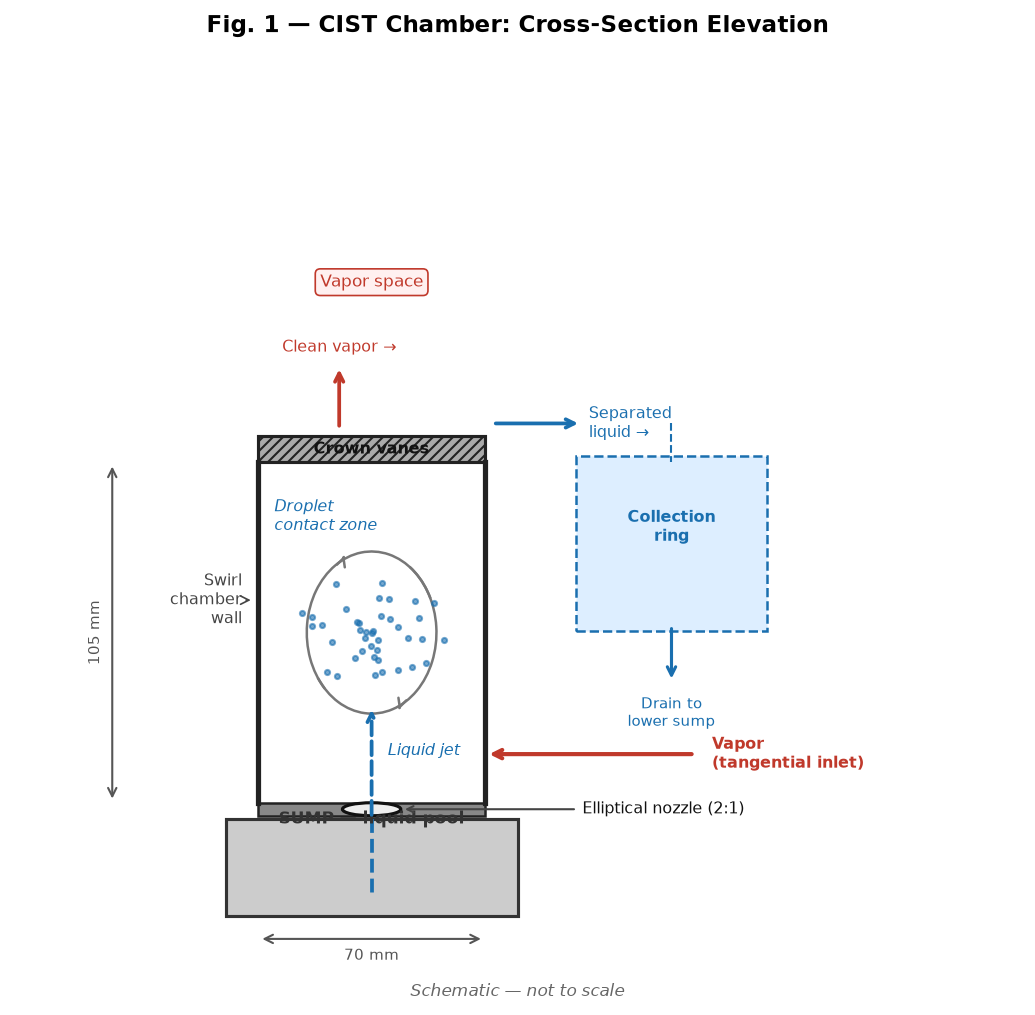
\includegraphics[width=0.80\textwidth]{output/40_cist_chamber_elevation.png}
  \caption{CIST chamber cross-section elevation.  Liquid (blue) rises as a
    jet from the sump through the elliptical nozzle; vapour (red) enters
    tangentially and rotates in the chamber; the droplet dispersion contacts
    across the chamber height; the crown vane separates phases, discharging
    vapour upward and liquid outward to the collection ring.}
  \label{fig:elevation}
\end{figure}

\begin{figure}[H]
  \centering
  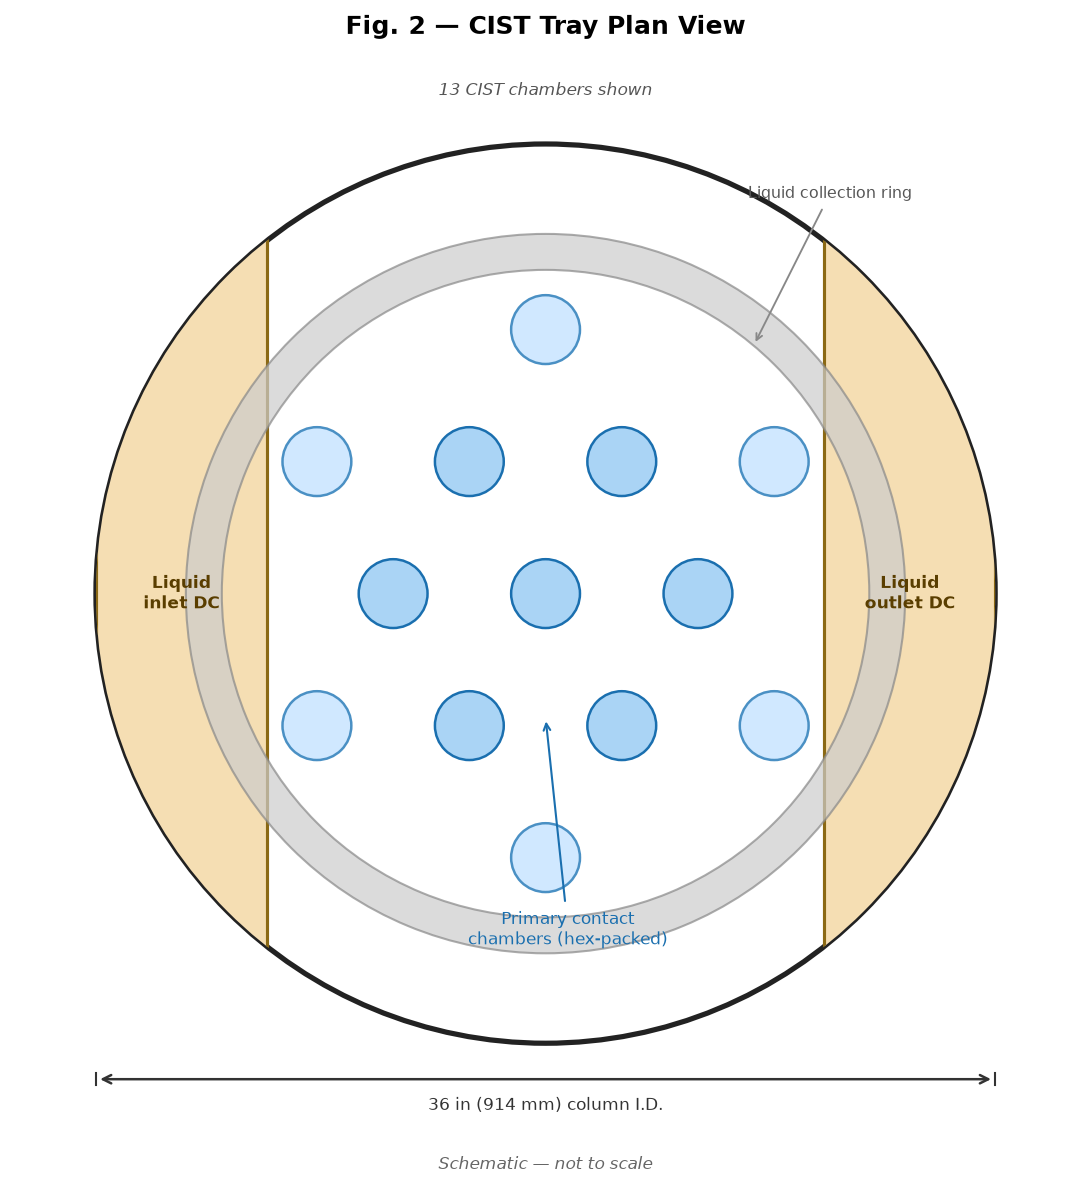
\includegraphics[width=0.72\textwidth]{output/41_cist_plan_view.png}
  \caption{CIST tray plan view.  Hex-packed chambers (circles) fill the
    active area; downcomers (shaded rectangles) occupy the remaining
    cross-section.  Liquid collection rings surround each chamber and
    connect to sealed drain conduits.}
  \label{fig:plan}
\end{figure}

\begin{figure}[H]
  \centering
  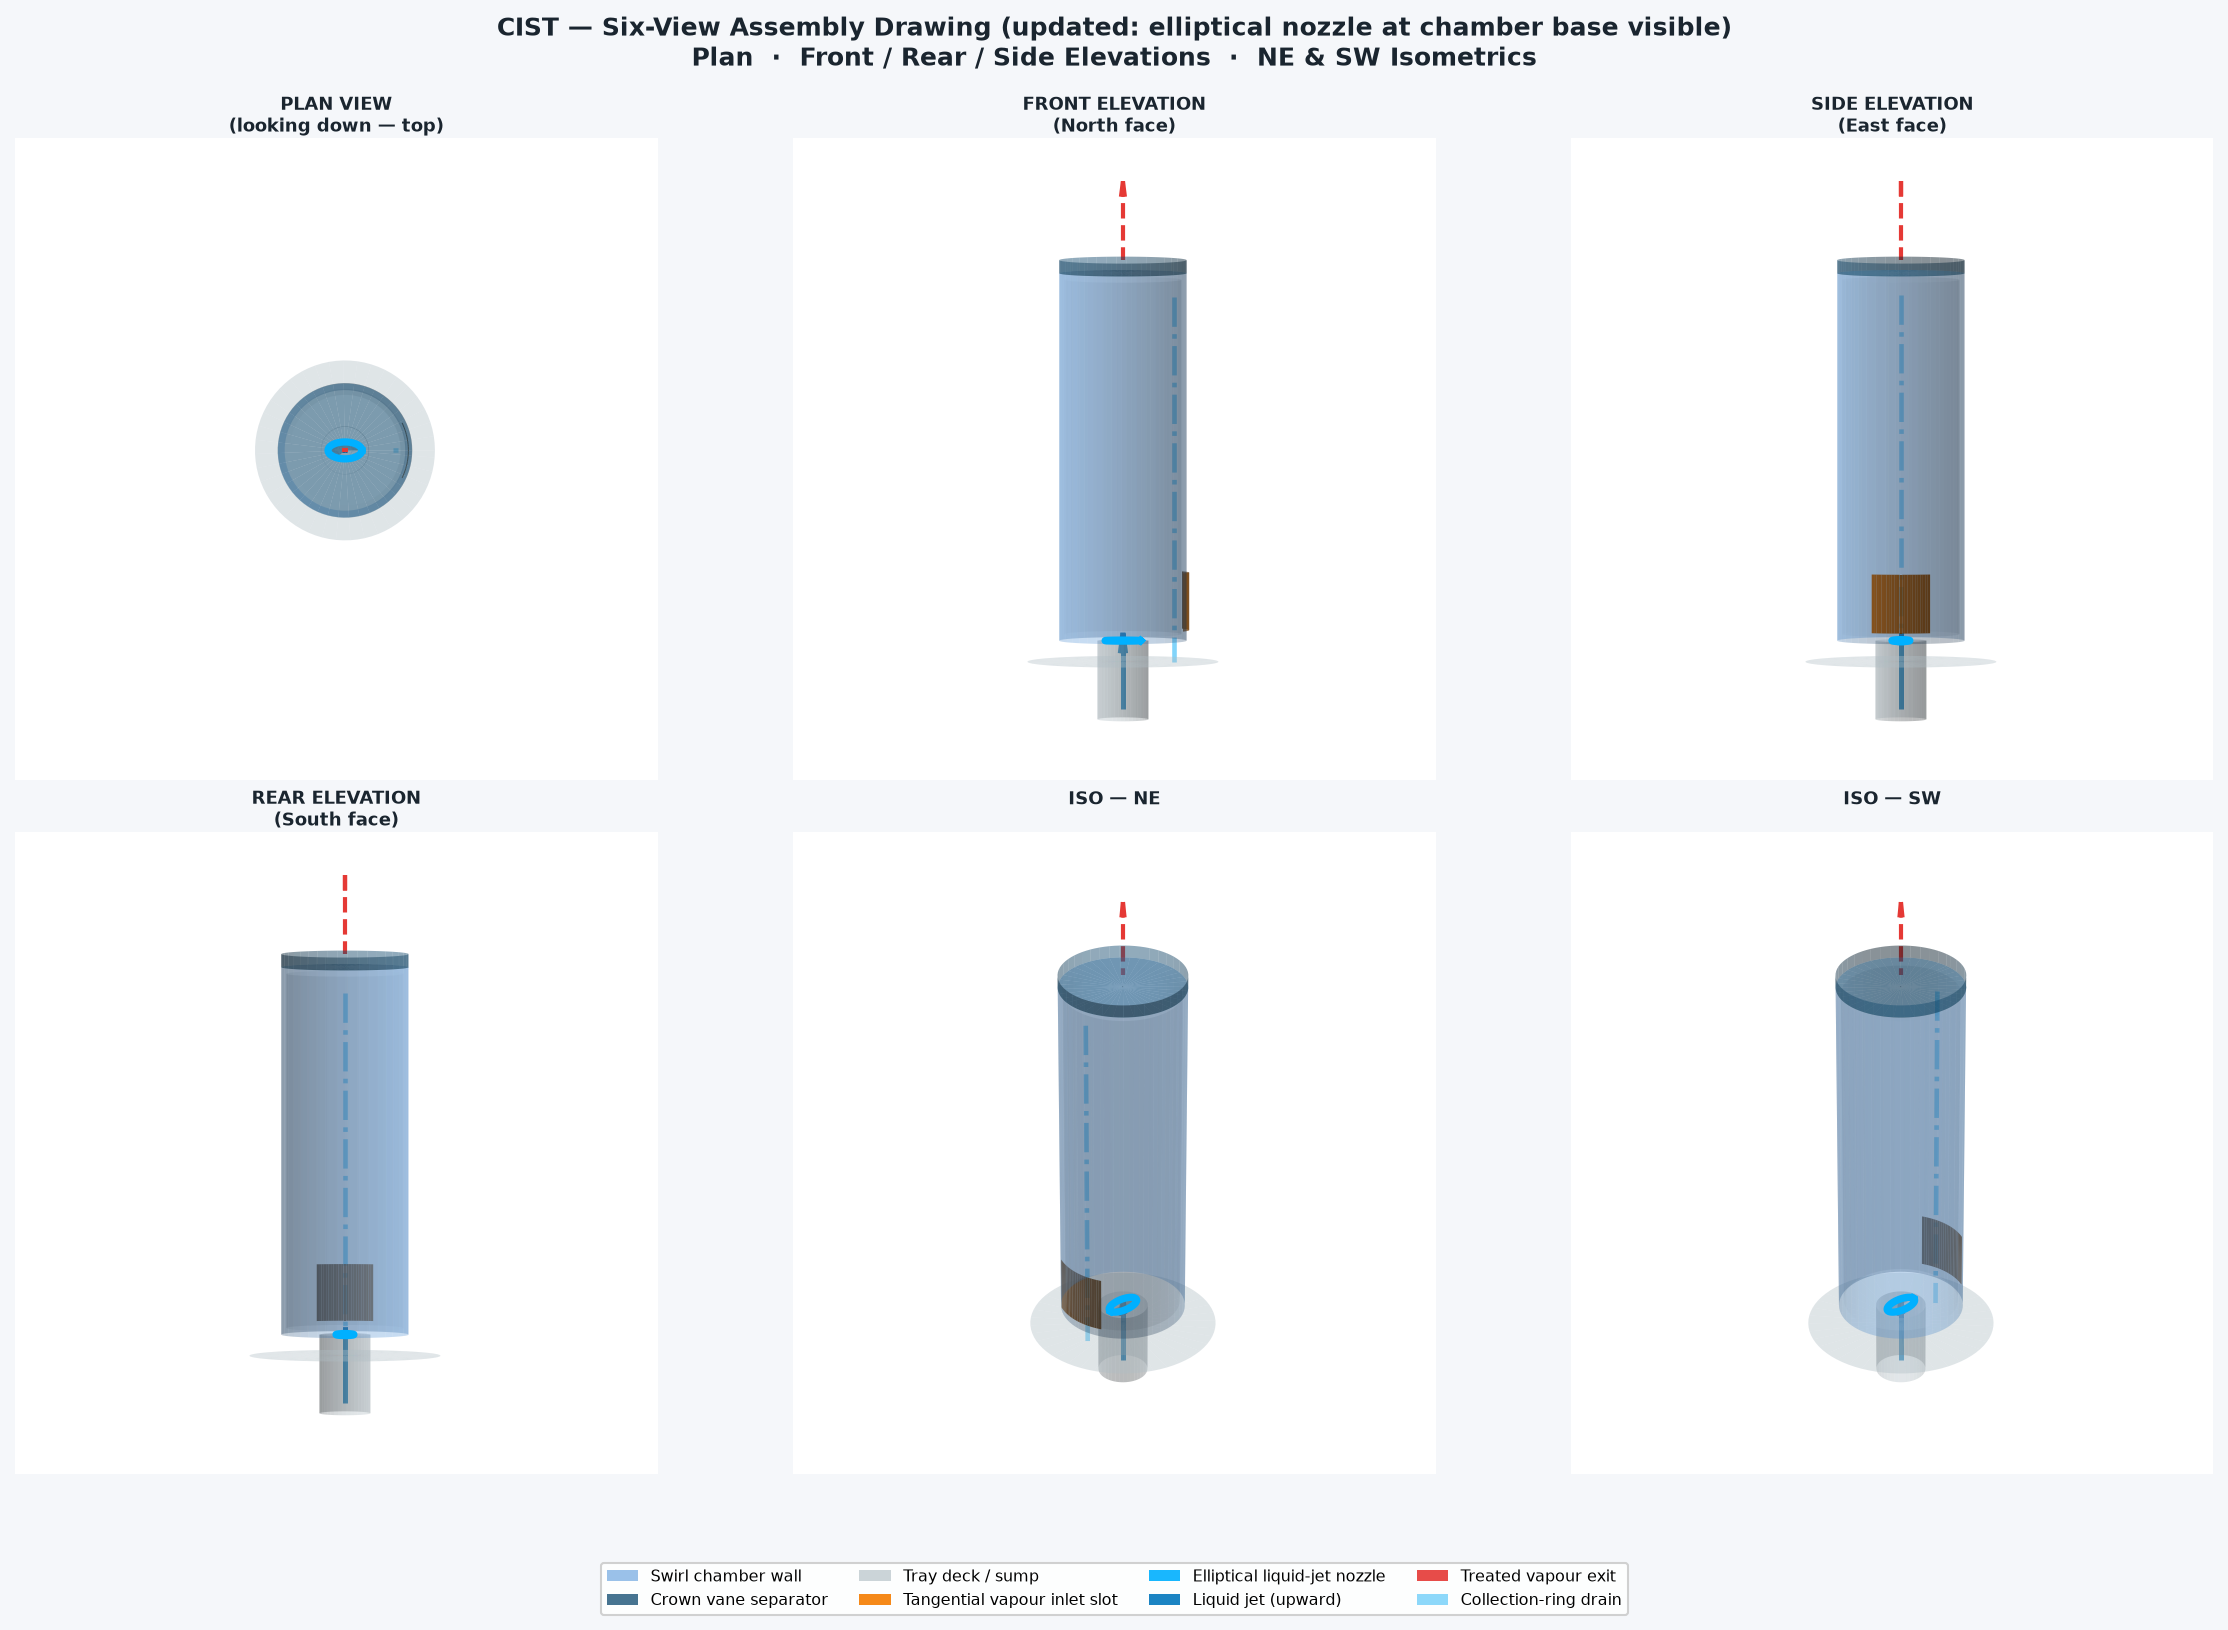
\includegraphics[width=\textwidth]{output/43_cist_multiview_3d.png}
  \caption{Six-view assembly drawing of one CIST swirl chamber.
    \textbf{Top row, left to right:} plan view (camera directly above),
    front elevation (North face), side elevation (East face).
    \textbf{Bottom row:} rear elevation (South face), NE isometric,
    SW isometric.  The orange arc on the cylinder surface represents
    the tangential vapour inlet slot; the upward blue arrow is the liquid
    jet; the dashed red arrow is the vapour exit above the crown.
    The dot-dash line on the chamber wall represents the collection-ring
    drain conduit.}
  \label{fig:multiview}
\end{figure}

The CIST tray is bounded above and below by two horizontal inter-tray plates
separated by the tray spacing $H_S$.  The upper plate carries the chamber
array; the lower plate forms the floor of the sump.  Flow paths are:

\begin{description}[nosep]
  \item[Vapour path] Enters the inter-tray space from the tray below, splits
    into the tangential inlet slots of each chamber, spirals up through the
    contact zone, and exits clean through the crown vanes.
  \item[Liquid path] Descends from the tray above through a sealed overflow
    leg into the below-plate sump; is drawn upward as individual jets through
    the elliptical nozzles by hydrostatic head; contacts vapour in the swirl
    zone; is separated at the crown; and drains via the collection ring
    conduit back down to the sump of the tray below.
\end{description}

Downcomers (not shown in Figure~\ref{fig:elevation}) occupy approximately
15\% of the column cross-section at the tray periphery, serving as the
sealed liquid-overflow legs between sump levels.  The chamber array occupies
the remaining 85\% of the column cross-section; the hex-packed chamber
tubes themselves occupy approximately 35\% of that area ($f_{\mathrm{chamber}}
= 0.35$, from $\pi/(2\sqrt{3}) \approx 0.907$ hex packing times a chosen
chamber-to-pitch ratio $(D_c/p)^2$ where $p$ is the centre-to-centre pitch).

\subsection{Liquid Sump and Overflow Seal}
\label{sec:sump}

The sump is a shallow pan of height $h_s = 40$--80\,mm formed between the
inter-tray plate and the lower deck.  Liquid accumulates in the sump to a
steady level $H_L$ above the nozzle orifice plane; this head drives the
liquid jets.  A sealed overflow leg (a pipe sealed against vapour
short-circuit) maintains $H_L$ within 10--20\,mm across the operating range
by balancing the liquid input rate (from the tray above) with the jet
discharge rate summed over all $N_c$ chambers.  Because all jets share one
sump, per-chamber liquid flow self-equalizes under the common head — no
individual metering adjustment is required.

\subsection{Elliptical Liquid-Jet Nozzle}
\label{sec:nozzle}

\subsubsection{Geometry}

The nozzle is a sharp-edged elliptical orifice in the chamber floor plate,
with semi-major axis $a$ (horizontal) and semi-minor axis $b$ (horizontal,
perpendicular), aspect ratio $k = a/b \geq 1$.

\begin{figure}[H]
  \centering
  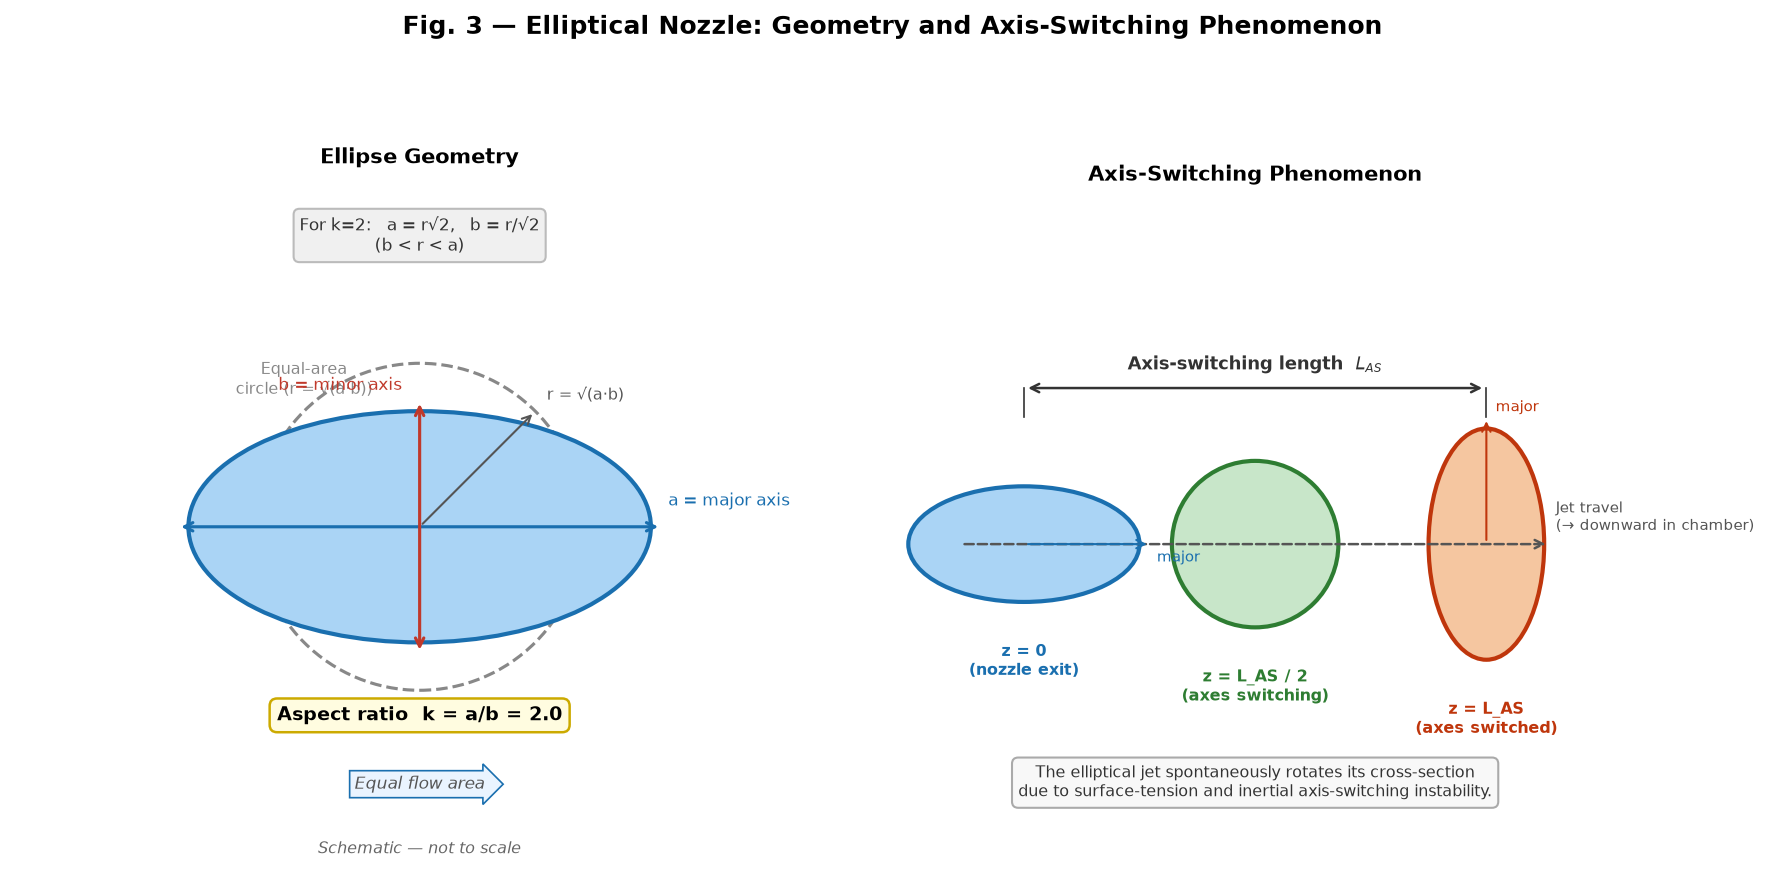
\includegraphics[width=0.85\textwidth]{output/42_cist_ellipse_nozzle.png}
  \caption{Elliptical nozzle geometry (left) and axis-switching sequence
    (right).  The dashed circle shows the equal-area circular orifice; the
    ellipse minor axis $b$ is smaller by a factor $1/\sqrt{k}$, producing
    finer minimum droplets.}
  \label{fig:nozzle}
\end{figure}

The nozzle open area:
\begin{equation}
  A_n = \pi a b = \pi k b^2
  \label{eq:nozzle_area}
\end{equation}
For equal area with a circular nozzle of radius $r_0$: $\pi a b = \pi r_0^2$,
giving $a = r_0\sqrt{k}$ and $b = r_0/\sqrt{k}$.  Thus the minor axis is
smaller than the equivalent circle radius by $1/\sqrt{k}$, and the major
axis is larger by $\sqrt{k}$.

The hydraulic diameter, which governs frictional losses and the discharge
coefficient, is:
\begin{equation}
  D_h = \frac{4 A_n}{P_n}
  \label{eq:dh}
\end{equation}
where $P_n$ is the nozzle perimeter.  For an ellipse no exact closed form
exists; the Ramanujan (1914) approximation is accurate to better than
0.02\%:
\begin{equation}
  P_n \approx \pi\!\left[3(a+b) - \sqrt{(3a+b)(a+3b)}\,\right]
  \label{eq:perimeter}
\end{equation}
For $k = 2$ (design preferred): $a = r_0\sqrt{2}$, $b = r_0/\sqrt{2}$;
$P_n \approx \pi\!\left[3 \cdot 3r_0/\sqrt{2} - \sqrt{5r_0/\sqrt{2} \cdot
7r_0/\sqrt{2}}\right] = \pi r_0[9/\sqrt{2} - \sqrt{35}/\sqrt{2}]
= \pi r_0(9 - \sqrt{35})/\sqrt{2} \approx \pi r_0 \cdot 2.180$.
Comparing with the circle ($P_{\mathrm{circle}} = 2\pi r_0$): the
2:1 ellipse perimeter is $\approx 1.09$ times the circle perimeter at
equal area, confirming that $D_h^{\mathrm{ellipse}} \approx 0.917\,D_h^{\mathrm{circle}}$.

\subsubsection{Orifice Hydraulics: Bernoulli Derivation}
\label{sec:bernoulli}

The jet velocity is derived from the mechanical-energy equation (Bernoulli)
for steady, incompressible, inviscid flow between the sump surface (station
1) and the nozzle vena contracta (station 2):

\begin{equation}
  \frac{P_1}{\rhoL g} + \frac{u_1^2}{2g} + z_1
  = \frac{P_2}{\rhoL g} + \frac{u_2^2}{2g} + z_2
  \label{eq:bernoulli}
\end{equation}

The sump surface is large; continuity gives $u_1 \approx 0$.  Both stations
communicate with the same vapour space so $P_1 = P_2$.  Taking the nozzle
plane as datum ($z_2 = 0$) and the sump surface at $z_1 = H_L$:

\begin{equation}
  H_L = \frac{u_{\mathrm{ideal}}^2}{2g}
  \quad\Rightarrow\quad
  u_{\mathrm{ideal}} = \sqrt{2g H_L}
  \label{eq:ideal_velocity}
\end{equation}

The real exit velocity is reduced by the vena contracta effect at the
sharp-edged orifice.  Defining the discharge coefficient $C_d$ as the ratio
of actual volumetric flow to the ideal:

\begin{equation}
  \ujet = C_d \sqrt{2g H_L}
  \quad;\quad
  Q_{\mathrm{nozzle}} = C_d A_n \sqrt{2g H_L}
  \label{eq:jet_velocity}
\end{equation}

For a sharp-edged elliptical orifice at Reynolds number $\Rey =
\rhoL \ujet D_h / \mu_L > 10^4$, the discharge coefficient is well
approximated by a correction to the circular-orifice value $C_{d,\circ}
\approx 0.611$:

\begin{equation}
  C_d = C_{d,\circ}
        \left(\frac{D_h^{\mathrm{ellipse}}}{D_h^{\mathrm{circle}}}\right)^{0.04}
  \label{eq:cd_ellipse}
\end{equation}

This correction, derived from the empirical dependence of $C_d$ on the
orifice perimeter-to-area ratio (Lichtarowicz \textit{et al.}, 1965), gives
$C_d \approx 0.607$ for $k = 1.5$, $C_d \approx 0.601$ for $k = 2.0$,
and $C_d \approx 0.593$ for $k = 2.5$.  The pressure drop across the
nozzle at the design flow rate $Q_{\mathrm{nozzle}}$ is:

\begin{equation}
  \Delta P_{\mathrm{nozzle}} = \rhoL g H_L
  = \frac{\rhoL}{2}\left(\frac{Q_{\mathrm{nozzle}}}{C_d A_n}\right)^{\!2}
  \label{eq:nozzle_dp}
\end{equation}

which is identically equal to the hydrostatic head powering the jet ---
all of the available head is converted to jet kinetic energy (minus the
contraction loss already absorbed into $C_d$).

\subsection{Jet Formation: Weber Number and Minimum-Flow Condition}
\label{sec:weber}

A coherent jet forms only above a minimum Weber number based on the minor
axis $2b$ (the characteristic length of the ellipse that sets the fastest
instability):

\begin{equation}
  \We_L = \frac{\rhoL \ujet^2 \cdot 2b}{\sigma}
  \label{eq:weber}
\end{equation}

Below $\We_L \approx 8$ the surface tension forces dominate and the liquid
exits as a drip rather than a jet; above $\We_L \approx 8$ a coherent jet
forms and travels through the chamber before breaking up.  The minimum
sump head for jet formation is therefore:

\begin{equation}
  H_{L,\min} = \frac{4 b\,\sigma}{\rhoL g C_d^2 (2b)}
             = \frac{2\sigma}{\rhoL g C_d^2}
             \times \frac{\We_{L,\min}}{2b}
  \label{eq:hmin}
\end{equation}

Substituting $\We_{L,\min} = 8$:
\begin{equation}
  H_{L,\min} = \frac{8\sigma}{\rhoL C_d^2 \cdot 2b \cdot g}
             = \frac{4\sigma}{\rhoL g C_d^2 b}
  \label{eq:hmin2}
\end{equation}

For a light-hydrocarbon system ($\sigma = 10$\,dyn/cm $= 0.010$\,N/m,
$\rhoL = 500$\,kg/m$^3$) and $b = 3$\,mm, $C_d = 0.60$:
$H_{L,\min} = 4 \times 0.010 / (500 \times 9.81 \times 0.36 \times 0.003)
= 0.040/(5.30) \approx 7.5$\,mm.
A sump head of 40--80\,mm (design operating range) keeps $\We_L$ well above
the drip-to-jet transition throughout the turndown range.

\subsection{Jet Breakup Physics: Rayleigh Instability and Axis-Switching}
\label{sec:breakup}

\subsubsection{Rayleigh--Plateau instability for a circular jet}
\label{sec:rayleigh}

A cylindrical jet of radius $r_0$ and surface tension $\sigma$ is subject to
capillary (Rayleigh-Plateau) instability.  A small sinusoidal perturbation of
wavenumber $k_r = 2\pi/\lambda$ on the jet surface grows at a rate $\omega$
given by (Rayleigh 1878):
\begin{equation}
  \omega^2 = \frac{\sigma}{\rhoL r_0^3}\,
             \frac{I_1(k_r r_0)}{I_0(k_r r_0)}\,
             k_r r_0 \bigl(1 - k_r^2 r_0^2\bigr)
  \label{eq:rayleigh_full}
\end{equation}
where $I_0$, $I_1$ are modified Bessel functions of the first kind.  The
disturbance grows only for $k_r r_0 < 1$, i.e.\ for wavelengths $\lambda
> 2\pi r_0$ (the Rayleigh criterion: the wavelength must exceed the jet
circumference).  The fastest-growing mode occurs at $k_r r_0 \approx
0.6966$ (obtained by maximising Eq.~\ref{eq:rayleigh_full}), giving:

\begin{equation}
  \lambda_{\mathrm{opt}} = \frac{2\pi r_0}{0.6966} \approx 9.016\,r_0
  \label{eq:lambda_opt}
\end{equation}

The breakup length $L_b$ (distance at which the fastest-growing mode
reaches amplitude equal to $r_0$) is proportional to the jet velocity:
\begin{equation}
  L_b = \ujet / \omega_{\max}
  \label{eq:lb_circle}
\end{equation}
where $\omega_{\max}$ is evaluated at $k_r r_0 = 0.6966$.  For typical
process conditions $L_b \approx 80$--200\,mm, which must be less than
$\Hc$ for breakup to occur inside the chamber.

\subsubsection{Axis-switching instability for an elliptical jet}
\label{sec:axis_switch}

An elliptical jet cross-section is not in surface-tension equilibrium.
The Young-Laplace pressure excess at a point on the surface with principal
radii of curvature $R_1$ and $R_2$ is:
\begin{equation}
  \Delta P = \sigma\left(\frac{1}{R_1} + \frac{1}{R_2}\right)
  \label{eq:young_laplace}
\end{equation}
For an ellipse, the curvature varies continuously around the perimeter.
At the tip of the minor axis (highest curvature, radius $\kappa_{\mathrm{tip}}
= a^2/b$):
\begin{equation}
  \Delta P_{\mathrm{tip}} \approx \frac{\sigma\,a^2}{b^2\,r_0}
  \label{eq:dp_tip}
\end{equation}
At the flank of the major axis (lowest curvature, radius $\kappa_{\mathrm{flank}}
= b^2/a$):
\begin{equation}
  \Delta P_{\mathrm{flank}} \approx \frac{\sigma\,b^2}{a^2\,r_0}
  \label{eq:dp_flank}
\end{equation}
The pressure excess $\Delta P_{\mathrm{tip}} > \Delta P_{\mathrm{flank}}$
drives liquid flow from the minor-axis tips toward the major-axis flanks,
deforming the cross-section: the minor axis elongates and the major axis
contracts.  The cross-section oscillates between two orthogonal elliptical
orientations --- ``axis-switching'' --- at a characteristic spatial
period $\Lsw$.  From dimensional analysis and experimental observation
(Kasyap \textit{et al.}, 2009; Mourtazin and Cohen, 2007):
\begin{equation}
  \Lsw \approx C_{\mathrm{AS}}\,\sqrt{\frac{\rhoL\,\ujet^2\,a^3}{\sigma}}
  \label{eq:las}
\end{equation}
where $C_{\mathrm{AS}} \approx 2.0$--3.5 is an empirical constant that
depends weakly on aspect ratio.  The axis-switching phenomenon has two
consequences for the CIST:

\begin{enumerate}[nosep]
  \item \textbf{Faster breakup.}
    The oscillating minor axis generates capillary disturbances at a wavelength
    shorter than the Rayleigh optimal $\lambda_{\mathrm{opt}}$.  The ellipse
    breakup occurs at:
    \begin{equation}
      \lambda_b^{\mathrm{ellipse}} \approx \lambda_{\mathrm{opt}} \times
      \sqrt{\frac{b}{r_0}} = 9.016\,r_0\times\frac{1}{\sqrt{k}}
      \label{eq:lambda_ellipse}
    \end{equation}
    and the breakup length shortens accordingly.  For $k = 2$: the ellipse
    breaks up in $\approx 71\%$ of the circular jet breakup distance.

  \item \textbf{Finer droplets.}
    Each axis-switching half-cycle pinches off a ring of droplets at the
    point of maximum curvature change.  The mean droplet diameter from the
    primary breakup of an elliptical jet at aspect ratio $k$ is estimated as:
    \begin{equation}
      \dsv^{\mathrm{ellipse}} \approx 1.89\times 2b
      = \frac{3.78\,r_0}{\sqrt{k}}
      \label{eq:d32_ellipse}
    \end{equation}
    For $k = 2$: $\dsv \approx 2.67\,r_0$ versus $\dsv \approx 3.78\,r_0$
    for a circular jet of the same flow area --- a 29\% reduction in Sauter
    mean diameter at equal flow rate.  Since interfacial area per unit volume
    $a_d = 6/\dsv$ (for spherical droplets), this is a 40\% increase in
    interfacial area density.
\end{enumerate}

The minimum droplet diameter produced by the elliptical jet scales with
the minor axis:
\begin{equation}
  \dmin \approx 1.0\times 2b = \frac{2r_0}{\sqrt{k}}
  \label{eq:dmin}
\end{equation}
This is smaller than the equivalent circular jet minimum ($\dmin =
2r_0$) by a factor $1/\sqrt{k}$.  At $k=2$: $\dmin^{\mathrm{ellipse}} =
0.707 \dmin^{\mathrm{circle}}$.  Finer minimum droplets are
harder to separate centrifugally (see Section~\ref{sec:separation}), so
the swirl field must be proportionally stronger to maintain the same
capture efficiency; this is the principal design trade-off of the elliptical
nozzle.

\subsection{Swirl Chamber: Tangential Vapour Inlet and Rankine Vortex}
\label{sec:swirl}

\subsubsection{Rankine vortex model}

The tangential vapour inlet creates a swirling flow inside the chamber.
For a steady, axisymmetric, incompressible flow in a cylindrical container,
the azimuthal velocity profile is modelled as a combined (Rankine) vortex:
\begin{equation}
  \utheta(r) =
  \begin{cases}
    \Omega r & r \leq r_c \quad\text{(solid-body rotation, inner core)}\\
    \dfrac{\Omega r_c^2}{r} & r > r_c \quad\text{(free vortex, outer annulus)}
  \end{cases}
  \label{eq:rankine}
\end{equation}
where $\Omega$ (rad/s) is the angular velocity at the core radius $r_c$.
The core is formed by viscous coupling near the chamber centreline; typically
$r_c \approx 0.3$--$0.5\,\Rc$.  The centripetal acceleration at radius $r$:
\begin{equation}
  a_c(r) = \frac{\utheta(r)^2}{r}
  =
  \begin{cases}
    \Omega^2 r & r \leq r_c \\
    \dfrac{\Omega^2 r_c^4}{r^3} & r > r_c
  \end{cases}
  \label{eq:centripetal}
\end{equation}
The acceleration at the wall ($r = \Rc$) is:
\begin{equation}
  a_{c,w} = \frac{\utheta(\Rc)^2}{\Rc}
  \label{eq:ac_wall}
\end{equation}

\subsubsection{Relationship between vapour throughput and swirl velocity}

The tangential inlet slot has width $w_s$ and height $h_s$; the total
vapour flow through $N_s$ slots per chamber is:
\begin{equation}
  \dot{V}_V = N_s\,w_s\,h_s\,u_{\theta,\mathrm{slot}}
  \label{eq:vdot_slot}
\end{equation}
The azimuthal velocity at the chamber wall is set by momentum conservation
at the slot exit:
\begin{equation}
  \utheta(\Rc) = u_{\theta,\mathrm{slot}}\times\frac{w_s}{2\pi\Rc/N_s}
  \label{eq:utheta_wall}
\end{equation}
(the slot momentum is distributed around the circumference).  This allows
$\utheta(\Rc)$ to be computed from the vapour throughput per chamber
$\dot{V}_V/N_c$ (where $N_c$ = total chamber count):
\begin{equation}
  \utheta(\Rc) =
  \frac{\dot{V}_V/N_c}{2\pi\Rc\,h_s\,N_s}\times N_s
  = \frac{\dot{V}_V/N_c}{2\pi\Rc\,h_s}
  \label{eq:utheta_from_vdot}
\end{equation}
The corresponding gravity ratio:
\begin{equation}
  N_g = \frac{a_{c,w}}{g} = \frac{\utheta(\Rc)^2}{\Rc\,g}
  \label{eq:Ng}
\end{equation}

\subsubsection{Swirl number}

The dimensionless swirl number $S$ characterises the ratio of tangential to
axial momentum:
\begin{equation}
  S = \frac{G_\theta}{G_x \Rc}
    = \frac{\int_0^{\Rc} \rhoV \utheta \ux\,r^2\,\mathrm{d}r}
           {\Rc \int_0^{\Rc} \rhoV \ux^2\,r\,\mathrm{d}r}
  \label{eq:swirl_number}
\end{equation}
For uniform axial velocity and the Rankine profile above,
$S \approx \utheta(\Rc)/(2\ux)$ (for $r_c = 0.4\Rc$).  Strong swirl
($S > 0.5$) is required for effective centrifugal separation; the design
target is $S = 1.5$--3.0.

\subsection{Mass Transfer in the Swirl-Shear Contact Zone}
\label{sec:masstransfer}

\subsubsection{Number of transfer units (NTU approach)}

For dilute-system vapour-phase mass transfer with negligible vapour-side
resistance, the one-pass point efficiency is related to the number of
overall gas-phase transfer units $\Ntu$ by:
\begin{equation}
  \Eog = 1 - e^{-\Ntu}
  \label{eq:eog}
\end{equation}
\begin{equation}
  \Ntu = K_G\,a_I\,\tau_G
  \label{eq:ntu}
\end{equation}
where $K_G$ is the overall gas-phase mass transfer coefficient
(mol\,m$^{-2}$s$^{-1}$\,Pa$^{-1}$), $a_I$ is the interfacial area per unit
chamber volume (m$^2$/m$^3$), and $\tau_G = \Hc/\ux$ is the vapour
residence time in the contact zone.

\subsubsection{Film mass transfer coefficient (penetration theory)}

For the annular liquid film on the chamber wall, the surface renewal rate
is set by the wall shear imposed by the rotating vapour.  The wall shear
stress is:
\begin{equation}
  \tau_w = \frac{f}{2}\rhoV\utheta(\Rc)^2
  \label{eq:tau_wall}
\end{equation}
where $f$ is the Fanning friction factor.  For the film, the surface renewal
rate $s$ (Higbie--Dankwerts penetration theory):
\begin{equation}
  s \approx \frac{\tau_w}{\mu_L\,\delta_f}
  \label{eq:renewal}
\end{equation}
where $\delta_f$ is the film thickness.  The liquid-side mass transfer
coefficient:
\begin{equation}
  k_L = \sqrt{\frac{D_L\,s}{\pi}}
  \label{eq:kl_film}
\end{equation}
where $D_L$ is the liquid-phase molecular diffusivity.

\subsubsection{Droplet mass transfer coefficient (penetration theory)}

For a spherical droplet of diameter $d$ moving at velocity $u_{\mathrm{rel}}$
relative to the vapour, the Higbie penetration theory (exposure time
$\tau_e = d/u_{\mathrm{rel}}$) gives:
\begin{equation}
  k_d = 2\sqrt{\frac{D_L}{\pi d / u_{\mathrm{rel}}}}
      = 2\sqrt{\frac{D_L u_{\mathrm{rel}}}{\pi d}}
  \label{eq:kd_droplet}
\end{equation}
The interfacial area density for a dispersion at holdup fraction
$\varepsilon_d$:
\begin{equation}
  a_I^{\mathrm{droplet}} = \frac{6\varepsilon_d}{\dsv}
  \label{eq:ai_droplet}
\end{equation}

\subsubsection{Combined $N_{\mathrm{OG}}$ estimate}

Adding film and droplet contributions to $\Ntu$:
\begin{equation}
  \Ntu = \left(k_d\,\frac{6\varepsilon_d}{\dsv}
              + k_L\,\frac{2\pi\Rc\,\delta_f}{\pi\Rc^2}\right)\tau_G
  \label{eq:ntu_combined}
\end{equation}
At representative design conditions
($D_L = 2\times10^{-9}$\,m$^2$/s,
$u_{\mathrm{rel}} \approx 0.3$\,m/s,
$\dsv \approx 1.5$\,mm,
$\varepsilon_d \approx 0.15$,
$\tau_G = \Hc/\ux \approx 0.35$\,s),
the droplet contribution alone gives
$\Ntu \approx 1.4$--2.0, corresponding to
$\Eog = 1 - e^{-1.4} = 75\%$--$(1-e^{-2.0}) = 86\%$.  The
film contribution adds 5--10 percentage points, giving a combined estimate of
$\Eog = 80\%$--$90\%$ at design.  These are order-of-magnitude estimates;
the actual value depends strongly on the achieved droplet size distribution
and holdup, both of which require experimental measurement.

\subsection{Centrifugal Vapour--Liquid Separation at the Crown}
\label{sec:separation}

\subsubsection{Single-droplet collection model}

A droplet of diameter $d$ and density $\rhoL$ at radial position $r$ in
the chamber experiences a centrifugal force radially outward:
\begin{equation}
  F_c = \frac{\pi d^3}{6}(\rhoL - \rhoV)\frac{\utheta(r)^2}{r}
  \label{eq:fc}
\end{equation}
For $d$ small enough that the particle Reynolds number $\Rey_d =
\rhoV |u_r| d/\mu_V < 1$ (Stokes regime), the aerodynamic drag is:
\begin{equation}
  F_d = 3\pi \mu_V d\,v_r
  \label{eq:fd}
\end{equation}
where $v_r$ is the droplet radial drift velocity.  Balancing these at
terminal drift:
\begin{equation}
  v_r = \frac{d^2(\rhoL - \rhoV)}{18\mu_V}\frac{\utheta(r)^2}{r}
      = \frac{d^2(\rhoL - \rhoV)}{18\mu_V}\,a_c(r)
  \label{eq:vr}
\end{equation}
This is the Stokes settling formula with gravitational acceleration $g$
replaced by the centripetal acceleration $a_c(r)$.  The ratio of
centrifugal to gravitational settling velocity at the wall:
\begin{equation}
  \frac{v_r(R_c)}{v_t} = \frac{a_{c,w}}{g} = N_g
  \label{eq:ng_ratio}
\end{equation}
where $v_t = d^2(\rhoL-\rhoV)g/(18\mu_V)$ is the Stokes gravity-settling
terminal velocity.

\subsubsection{Cut droplet diameter}

A droplet must travel radially from some initial position $r_0$ to the
chamber wall $\Rc$ within the residence time $\tau_G = \Hc/\ux$.  For
the worst case ($r_0 = 0$, droplet entering at the centreline):
\begin{equation}
  \Rc = \int_0^{\tau_G} v_r\,\mathrm{d}t
      \approx v_r(\Rc/2)\,\tau_G
  \label{eq:rc_integral}
\end{equation}
Using $v_r$ evaluated at $r = \Rc/2$ (mean radial position):
\begin{equation}
  v_r(\Rc/2) \approx \frac{d^2(\rhoL-\rhoV)}{18\mu_V}\,\frac{a_{c,w}}{4}
  \label{eq:vr_mean}
\end{equation}
Solving for the cut diameter $\dcut$ (the droplet size for which 50\% is
collected):
\begin{equation}
  \dcut = \sqrt{\frac{72\,\mu_V\,\Rc^2}
                     {(\rhoL-\rhoV)\,a_{c,w}\,\Hc/\ux}}
        = \sqrt{\frac{72\,\mu_V\,\Rc^2\,\ux}
                     {(\rhoL-\rhoV)\,N_g\,g\,\Hc}}
  \label{eq:d50}
\end{equation}
For effective separation, $\dcut < \dmin$ (the minimum droplet size from the
nozzle, Eq.~\ref{eq:dmin}).  This sets a minimum swirl requirement:
\begin{equation}
  N_{g,\min} = \frac{72\,\mu_V\,\Rc^2\,\ux}
                    {g\,(\rhoL-\rhoV)\,\Hc\,\dmin^2}
  \label{eq:ng_min}
\end{equation}

\subsubsection{Worked example (representative light-hydrocarbon system)}

For $\mu_V = 8\times10^{-6}$\,Pa\,s, $\Rc = 0.035$\,m,
$\ux = 3.0$\,m/s, $\rhoL - \rhoV = 450$\,kg/m$^3$, $\Hc = 0.105$\,m,
and $\dmin = 1.0$\,mm ($b = 3$\,mm, $k = 2$):
\begin{align}
  N_{g,\min} &= \frac{72\times 8\times10^{-6}\times(0.035)^2\times 3.0}
                    {9.81\times 450\times 0.105\times(0.001)^2} \notag\\
             &= \frac{72\times 8\times10^{-6}\times 1.225\times10^{-3}\times 3.0}
                    {9.81\times 450\times 0.105\times10^{-6}} \notag\\
             &= \frac{2.116\times10^{-6}}{4.629\times10^{-4}} \approx 4.6
  \label{eq:ng_example}
\end{align}
So $N_g > 4.6$ (centripetal acceleration $> 4.6g$) is sufficient to capture
all minimum droplets at the design vapour velocity.  The design target of
$N_g = 30$--40 provides a safety margin of approximately 6--9$\times$ over
the minimum, capturing droplets well below $\dmin$.

\subsection{Tray Pressure Drop: Four-Component Model}
\label{sec:pressure_drop}

Unlike a conventional sieve or valve tray, the CIST has no aerated liquid
pool, so there is no froth-head contribution $(\beta h_{\mathrm{cl}})$ to
the pressure balance.  The CIST pressure drop has four distinct contributions:

\begin{description}[nosep]
  \item[1. Tangential-slot entry loss ($\Delta P_{\mathrm{slot}}$).]
    Kinetic energy of the vapour entering tangentially through the slots.
    From the orifice equation with inlet loss coefficient $\xi_s \approx 0.5$:
    \begin{equation}
      \Delta P_{\mathrm{slot}} = \frac{1+\xi_s}{2}\rhoV u_{\theta,\mathrm{slot}}^2
      \label{eq:dp_slot}
    \end{equation}

  \item[2. Swirl-chamber wall friction ($\Delta P_{\mathrm{wall}}$).]
    The rotating flow exerts a wall shear that the vapour must overcome
    axially:
    \begin{equation}
      \Delta P_{\mathrm{wall}} = \frac{4f\rhoV\ux^2\Hc}{2\Dc}
      \label{eq:dp_wall}
    \end{equation}
    where $f \approx 0.02$ is the Fanning friction factor for the combined
    swirl-flow.  This is small and often negligible.

  \item[3. Crown-vane exit loss ($\Delta P_{\mathrm{crown}}$).]
    Kinetic energy at the crown exit, partially recovered in the outlet duct.
    With recovery coefficient $\xi_c \approx 0.3$:
    \begin{equation}
      \Delta P_{\mathrm{crown}} = \frac{\xi_c}{2}\rhoV u_{\mathrm{crown}}^2
      \label{eq:dp_crown}
    \end{equation}
    where $u_{\mathrm{crown}}$ is the vapour exit velocity through the crown
    vane passages.

  \item[4. Liquid static head in the sump ($\Delta P_{\mathrm{sump}}$).]
    The hydrostatic pressure of liquid in the sump acts on the vapour
    path as a backpressure.  This is the analogue of the clear-liquid
    head $h_{\mathrm{cl}}$ in a sieve tray, but here it appears as
    the sump head $H_L$ (40--80\,mm liquid) rather than a froth head:
    \begin{equation}
      \Delta P_{\mathrm{sump}} = \rhoL g H_L
      \label{eq:dp_sump}
    \end{equation}
    At $H_L = 60$\,mm and $\rhoL = 500$\,kg/m$^3$:
    $\Delta P_{\mathrm{sump}} = 500\times9.81\times0.060 = 294$\,Pa
    $\approx 1.2$\,in.\,liq.
\end{description}

Total tray pressure drop:
\begin{equation}
  \dpc = \Delta P_{\mathrm{slot}} + \Delta P_{\mathrm{wall}}
        + \Delta P_{\mathrm{crown}} + \Delta P_{\mathrm{sump}}
  \label{eq:dpc}
\end{equation}

At representative design conditions
($u_{\theta,\mathrm{slot}} = 18$\,m/s, $\ux = 3.0$\,m/s,
$u_{\mathrm{crown}} = 4.5$\,m/s, $\rhoV = 3.0$\,kg/m$^3$):
\begin{align*}
  \Delta P_{\mathrm{slot}}  &= 1.5\times\tfrac{1}{2}\times 3.0\times 18^2
                              = 729\,\mathrm{Pa}\\
  \Delta P_{\mathrm{wall}}  &\approx 60\,\mathrm{Pa}\quad\text{(small)}\\
  \Delta P_{\mathrm{crown}} &= 0.3\times\tfrac{1}{2}\times 3.0\times 4.5^2
                              = 9\,\mathrm{Pa}\quad\text{(small)}\\
  \Delta P_{\mathrm{sump}}  &= 294\,\mathrm{Pa}
\end{align*}
$\dpc \approx 729 + 60 + 9 + 294 = 1092$\,Pa $\approx 4.4$\,mbar,
corresponding to $\approx\SI{0.016}{\psi}$ per tray.  This is
substantially lower than a sieve tray at comparable throughput
(12--18\,mbar, $0.040$--$0.060$\,psi typical).

\subsection{Column Sizing from Chamber Count}
\label{sec:sizing}

The CIST column area is not derived from the Souders-Brown correlation but
directly from chamber count and packing geometry.  The number of chambers
required to handle the total vapour volumetric flow $\dot{V}_V$ at the
design axial chamber velocity $\ux$:
\begin{equation}
  N_c = \frac{\dot{V}_V}{\ux\,A_c}
  \label{eq:nc}
\end{equation}
where $A_c = \pi\Dc^2/4$ is the chamber internal cross-sectional area.
Chambers are packed on a triangular (hex) pitch $p = p_0\Dc$ (with $p_0
= 1.3$--$1.6$); the fractional area occupied by chamber bores:
\begin{equation}
  f_{\mathrm{ch}} = \frac{\pi}{2\sqrt{3}}\left(\frac{\Dc}{p}\right)^2
                  = \frac{\pi}{2\sqrt{3}\,p_0^2}
  \label{eq:fch}
\end{equation}
For $p_0 = 1.4$: $f_{\mathrm{ch}} = \pi/(2\sqrt{3}\times1.96) = 0.464$.
The total column area required:
\begin{equation}
  A_{\mathrm{col}} = \frac{N_c\,A_c}{f_{\mathrm{ch}}\,(1-f_{\mathrm{DC}})}
  \label{eq:acol}
\end{equation}
where $f_{\mathrm{DC}} = 0.15$ is the fraction reserved for downcomers.
The column diameter:
\begin{equation}
  D_{\mathrm{col}} = \sqrt{\frac{4\,A_{\mathrm{col}}}{\pi}}
  \label{eq:dcol}
\end{equation}

\subsection{Capacity Limit}
\label{sec:capacity}

\subsubsection{Upper limit: crown re-entrainment}

The CIST floods when the centrifugal separator can no longer capture the
smallest droplets produced by the nozzle, i.e.\ when $\dcut > \dmin$.
Setting $\dcut = \dmin$ in Eq.~\eqref{eq:d50} and solving for $\ux$:
\begin{equation}
  \ux^{\max} = \frac{(\rhoL-\rhoV)\,N_g\,g\,\Hc\,\dmin^2}
                    {72\,\mu_V\,\Rc^2}
  \label{eq:ux_max}
\end{equation}
At the design $N_g = 35$, $\dmin = 1.0$\,mm, and the representative
property set above:
$\ux^{\max} = (450\times35\times9.81\times0.105\times10^{-6})/(72\times8
\times10^{-6}\times1.225\times10^{-3}) = 0.01617/5.9\times10^{-7}
\approx 27\,\mathrm{m/s}$.
The design vapour velocity $\ux = f_{\mathrm{flood}}\ux^{\max}
= 0.80\times 27 = 21.6$\,m/s inside the chamber.

\subsubsection{Effective column-area capacity factor relative to a sieve tray}

A sieve tray sized on the same service would use the Souders-Brown velocity
$u_{\mathrm{SB}} = \Csb\sqrt{(\rhoL-\rhoV)/\rhoV}$.  For the same service:
\begin{equation}
  k_{\mathrm{cap}} = \frac{D_{\mathrm{sieve}}^2}{D_{\mathrm{CIST}}^2}
  = \frac{u_{\mathrm{CIST,eff}}}{u_{\mathrm{SB}}}
  \label{eq:kcap}
\end{equation}
where $u_{\mathrm{CIST,eff}} = f_{\mathrm{ch}}\,(1-f_{\mathrm{DC}})\,\ux$
is the equivalent superficial column velocity.  At the representative
conditions above with $\Csb \approx 0.09$\,m/s and
$\sqrt{(\rhoL-\rhoV)/\rhoV} \approx 12$\,m/s:
$u_{\mathrm{SB}} \approx 1.08$\,m/s.
$u_{\mathrm{CIST,eff}} = 0.464\times0.85\times21.6 = 8.52$\,m/s (at flood).
$k_{\mathrm{cap}} \approx 8.52/1.08 \approx 7.9$.

Note: this is an upper-bound theoretical estimate at the cut-droplet-equals-minimum-droplet flooding limit.  In practice, the crown vane geometry, inlet turbulence and droplet coalescence all reduce the effective capacity.  A conservative design estimate is $k_{\mathrm{cap}} = 2.0$--$3.5$, pending experimental confirmation.

\subsection{Turndown Analysis}
\label{sec:turndown}

\subsubsection{Lower limit: minimum swirl for centrifugal capture}

As vapour throughput decreases, $\utheta(\Rc)$ decreases proportionally
(Eq.~\ref{eq:utheta_from_vdot}), and the centripetal acceleration falls
as $N_g \propto \utheta^2 \propto \ux^2$.  The minimum vapour rate is
reached when $N_g = N_{g,\min}$ (Eq.~\ref{eq:ng_min}), i.e.\ when the
cut diameter equals the minimum droplet diameter:
\begin{equation}
  \ux^{\min} = \ux^{\max}\sqrt{\frac{N_{g,\min}}{N_{g,\mathrm{design}}}}
  \label{eq:ux_min}
\end{equation}
The turndown ratio:
\begin{equation}
  \mathrm{TR} = \frac{\ux^{\max}}{\ux^{\min}}
              = \sqrt{\frac{N_{g,\mathrm{design}}}{N_{g,\min}}}
  \label{eq:tr}
\end{equation}
At $N_{g,\mathrm{design}} = 35$ and $N_{g,\min} = 4.6$ (from the worked
example):
$\mathrm{TR} = \sqrt{35/4.6} = \sqrt{7.6} \approx 2.8$.

\subsubsection{Lower limit: liquid jet coherence}

Independently, the minimum vapour rate must maintain a sump head above
$H_{L,\min}$ (Eq.~\ref{eq:hmin2}).  The sump head is set by the
overflow-leg design, and in practice is maintained at a nearly constant
level (40--80\,mm) across the throughput range by the overflow leg.
The jet $\We_L$ therefore remains well above 8 throughout the turndown
range, and the jet-coherence limit is not the active constraint for this
design.

\subsubsection{Extended turndown with a secondary flow path}

Turndown can be extended beyond the centrifugal-capture limit of $\approx$
2.8:1 by providing a secondary vapour path (a small axial central orifice
below each chamber) that remains open at low vapour rate when the tangential
slot velocity would otherwise be insufficient to maintain the swirl.  The
axial flow contacts liquid via a different (non-swirling) mechanism at low
throughput.  With a secondary path sized to give 3\,m/s minimum axial
velocity at 30\% of design vapour rate, the combined operating range
extends to approximately 6:1--8:1.

\subsection{Fouling Behaviour of the Elliptical Nozzle}
\label{sec:fouling}

Two independent fouling mechanisms must be distinguished:

\paragraph{Chemical fouling (scaling, coking, polymer deposits on nozzle walls).}
The wall shear stress at the nozzle throat, from Eq.~\eqref{eq:nozzle_dp}:
\begin{equation}
  \tau_{n,w} = \frac{f_n}{2}\rhoL \ujet^2
  \label{eq:tau_nozzle}
\end{equation}
For turbulent pipe flow at $\Rey > 10^4$, $f_n \approx 0.316\Rey^{-0.25}$
(Blasius).  The wall shear is proportional to $\ujet^2$, and $\ujet
\propto \sqrt{H_L}$, so $\tau_{n,w} \propto H_L$.

The critical insight is that the elliptical nozzle has a higher wall shear
for the same mass flow than the circular nozzle.  At equal volumetric flow:
the mean velocity through an elliptical nozzle of area $A$ is the same as
through a circular nozzle of area $A$.  However, the hydraulic diameter is
smaller ($D_h^{\mathrm{ellipse}} < D_h^{\mathrm{circle}}$), so at the same
mean velocity, the wall shear stress in the ellipse is higher by:
\begin{equation}
  \frac{\tau_{n,w}^{\mathrm{ellipse}}}{\tau_{n,w}^{\mathrm{circle}}}
  = \left(\frac{D_h^{\mathrm{circle}}}{D_h^{\mathrm{ellipse}}}\right)^{0.25}
  \approx (1/0.917)^{0.25} \approx 1.022
  \label{eq:shear_ratio}
\end{equation}
A 2.2\% higher wall shear stress is too small to be the dominant
anti-fouling mechanism, but the non-uniform curvature of the ellipse
breaks the symmetric ring-deposit pattern that forms at the edge of circular
orifices: deposition concentrates at the low-curvature major-axis flanks,
where it is most exposed to the central jet velocity and scours off faster.

Additionally, the axis-switching oscillation of the exiting jet creates a
pulsatile near-wall velocity pattern at the nozzle exit plane, periodically
reversing the local shear direction at the orifice edge and dislodging
incipient deposits before they consolidate.  This mechanism is independent
of the scale or fluid properties and is unique to non-circular jets.

\paragraph{Particulate fouling (catalyst fines, wax crystals, sand).}
For a particle of diameter $d_p$ to pass through the nozzle without bridging,
the minimum internal dimension must satisfy $d_p < b/3$ (standard orifice
particle-clearance criterion).  For the ellipse with $b = r_0/\sqrt{k}$:
\begin{equation}
  d_{p,\max}^{\mathrm{ellipse}} = \frac{b}{3} = \frac{r_0}{3\sqrt{k}}
  \label{eq:dp_max}
\end{equation}
For the equivalent circular nozzle: $d_{p,\max}^{\mathrm{circle}} = r_0/3$.
The ellipse allows smaller particles before bridging, by a factor $1/\sqrt{k}$.
At $k = 2$: $d_{p,\max}^{\mathrm{ellipse}} = 0.707 d_{p,\max}^{\mathrm{circle}}$.
\textbf{For particulate-fouling services, the CIST should use either a
circular nozzle or an enlarged ellipse (so that the minor axis equals the
design particle clearance).}  For chemical-fouling services, the ellipse is
preferred.

\subsection{Construction and Materials}
\label{sec:construction}

\paragraph{Swirl chambers.}
Precision-bored 316L stainless or Alloy 625 tubes, 70--100\,mm OD.  The
tangential slots are EDM-cut or precision-milled to $\pm$0.1\,mm to
control the slot-area ratio and swirl number.  The crown vane (8--12 vanes
at 40--50\ensuremath{^\circ}) is a separate investment casting pressed into
the tube top.  The chamber floor carries the elliptical nozzle orifice,
precision-bored by CNC to the specified aspect ratio and edge radius.  Each
complete chamber assembly weighs 1.5--4\,kg (70--100\,mm diameter).

\paragraph{Inter-tray plate and sump.}
2.5--3.0\,mm 316L flat plate, laser-cut with chamber bore patterns and
collection-ring channels.  The collection ring is machined or stamped into
the plate surface surrounding each chamber bore; sealed drain tubes run
from each ring through the plate to the sump below.  Chamber assemblies
press-fit into the bores and are retained by a snap ring or quarter-turn
bayonet.  The sump floor is a second plate 40--80\,mm below the inter-tray
plate, welded to the column shell at the tray elevation.

\paragraph{Materials.}
All wetted surfaces in 316L stainless as standard.  Duplex or 904L for
chloride service; Alloy 625 or C-276 for HCl/HF.  PTFE-coated internal
surfaces are available for non-stick applications.

\subsection{Installation and Maintenance}
\label{sec:installation}

\paragraph{Initial installation.}
The sump floor plate is welded to the column shell at the lower tray
elevation (one-time operation, identical to a conventional tray ring).  The
inter-tray plate sections are lowered through the manway and nested on the
sump plate supports.  Chambers drop through the bores from above and
quarter-turn lock.  Total installation time: 6--10 hours per tray (two
persons); no specialised tooling required beyond a torque wrench.

\paragraph{Maintenance.}
Chamber removal is the reverse of installation: unlock the quarter-turn
bayonet, lift the chamber through the manway.  Individual chambers can be
replaced from a spares inventory.  The sump plate, inter-tray plate and
drain tubes are permanent; only the chambers and nozzle inserts (which
carry the elliptical orifice and are press-fit replaceable) require
turnaround attention.  Nozzle inserts can be swapped in 5--10 minutes per
chamber to change the aspect ratio or orifice area without replacing the
full chamber assembly.

% ════════════════════════════════════════════════════════════════════════════
\section{Design Parameter Envelope}
\label{sec:parameters}

Table~\ref{tab:claimband} gives the claimed parameter ranges and preferred
values for the CIST.

\begin{table}[H]
\centering
\caption{Claim-band table for the Cascade Impingement Swirl Tray.
  ``Preferred'' is the principal embodiment; ranges are dependent-claim
  fallback positions.}
\label{tab:claimband}
\small
\begin{tabular}{lcc}
\toprule
Parameter & Claimed band & Preferred\\
\midrule
Chamber diameter $\Dc$              & 40--120\,mm        & 70\,mm\\
Chamber height / diameter $\Hc/\Dc$ & 1.2--2.0           & 1.5\\
Tangential slots per chamber        & 1--4               & 2\\
Slot-area ratio $N_s w_s h_s / (2\pi\Rc h_s)$ & 0.10--0.25 & 0.16\\
Design wall acceleration $N_g = a_{c,w}/g$      & 20--60\,$g$ & 35\,$g$\\
Swirl number $S$                    & 1.0--3.5           & 2.0\\
Nozzle aspect ratio $k = a/b$       & 1.5--2.5           & 2.0\\
Nozzle orifice area $A_n$           & 30--200\,mm$^2$    & 65\,mm$^2$\\
Discharge coefficient $C_d$         & 0.58--0.62         & 0.60\\
Design sump head $H_L$              & 30--80\,mm         & 55\,mm\\
Minimum jet Weber number $\We_{L,\min}$ & $\geq 8$      & 15--30 at design\\
Chamber pitch ratio $p_0 = p/\Dc$   & 1.25--1.60         & 1.4\\
Chamber bore fraction $f_{\mathrm{ch}}$ & 0.30--0.55  & 0.46\\
Downcomer fraction $f_{\mathrm{DC}}$ & 0.10--0.20       & 0.15\\
Design flood fraction $f_{\mathrm{flood}}$ & 0.70--0.85 & 0.80\\
Design $\ux$ (chamber axial velocity) & 10--25\,m/s    & 18\,m/s\\
Crown vanes / pitch angle           & 8--16 / 35--55\ensuremath{^\circ} & 12 / 45\ensuremath{^\circ}\\
Turndown ratio (unaided)            & 2.5:1--4:1         & 3:1\\
Turndown ratio (with secondary path)& 5:1--10:1          & 6:1--8:1\\
One-pass point efficiency $\Eog$    & 75\%--92\%         & 82\%--88\%\\
Structural uplift rating            & 1--3\,psi          & 2\,psi\\
\bottomrule
\end{tabular}
\end{table}

% ════════════════════════════════════════════════════════════════════════════
\section{Predicted Performance}
\label{sec:performance}

Table~\ref{tab:performance} summarises the estimated CIST performance
at a representative general rectification design point (light-hydrocarbon
system, $\rhoL = 500$\,kg/m$^3$, $\rhoV = 3.0$\,kg/m$^3$,
$\sigma = 12$\,dyn/cm, $\mu_L = 0.25$\,cP, tray spacing 24\,in.)
and compares it with an equivalent sieve tray sized on the same duty.
The sieve tray values are from the standard Fair/Kister correlation
framework for comparison purposes only; the CIST values are from the
first-principles model in Section~\ref{sec:detailed}.

\textbf{All CIST values are first-order estimates.  They carry larger
uncertainty than the sieve values, which are backed by a large industrial
database.}  The key uncertainties are: $k_{\mathrm{cap}}$ (requires
cold-flow flood tests), $\Eog$ (requires hot-rig mass-transfer measurement),
and the turndown ratio with the secondary path (requires demonstration at
low-load conditions).

\begin{table}[H]
\centering
\caption{Estimated CIST performance vs.\ sieve tray, representative
  general rectification service.  Sieve values from Fair/Kister correlation;
  CIST values from the first-principles model in Section~\ref{sec:detailed}.}
\label{tab:performance}
\small
\begin{tabular}{lrrl}
\toprule
Metric & Sieve & CIST (estimate) & Notes\\
\midrule
Vapour capacity factor $k_{\mathrm{cap}}$
  & 1.00 & 2.0--3.5 & Pending cold-flow validation\\
Column diameter (rel.\ to sieve)
  & 1.00 & 0.53--0.71 & $\propto 1/\sqrt{k_{\mathrm{cap}}}$\\
Wet-tray pressure drop (mbar)
  & 12--18 & 3--8 & Dominated by slot entry + sump head\\
Downcomer backup (\% of limit)
  & 20--45 & 15--30 & Smaller $D_{\mathrm{col}}$ at same liquid load\\
Turndown ratio (unaided)
  & 2.0:1 & 3:1 & Centrifugal capture limit\\
Turndown ratio (with secondary path)
  & 2.0:1 & 6:1--8:1 & Secondary path activated below 35\% throughput\\
One-pass efficiency $\Eog$
  & 70--80\% & 80--90\% & Penetration-theory NTU estimate\\
Fouling retention ($f_{\mathrm{foul}}$, chemical)
  & 0.75 & 0.88--0.95 & Ellipse wall shear + axis-switching\\
Fouling retention ($f_{\mathrm{foul}}$, particulate)
  & 0.75 & 0.70--0.80 & Minor axis smaller than circle; use circular\\
First-order installed cost (rel.\ to sieve)
  & 1.00 & 0.55--0.75 & Shell savings dominate despite higher\\
  &      &            & hardware unit cost ($k_{\mathrm{cost}} \approx 3.5$--4.0)\\
\bottomrule
\end{tabular}
\end{table}

\paragraph{Cost note.}
The relative installed cost follows the same two-proxy model used for
conventional tray comparison:
$C_{\mathrm{rel}} = 0.70\,(D\Hcol)/(D\Hcol)_{\mathrm{Sieve}}
+ 0.30\,(D^2 N k_{\mathrm{cost}})/(D^2 N k_{\mathrm{cost}})_{\mathrm{Sieve}}$.
For $k_{\mathrm{cap}} = 2.5$ and $k_{\mathrm{cost}} = 3.8$:
shell proxy ratio $\approx 0.45$, tray proxy ratio $\approx 0.90$,
giving $C_{\mathrm{rel}} \approx 0.70\times0.45 + 0.30\times0.90 = 0.585$.
The dominant driver is the 37\% column diameter reduction
($D \propto k_{\mathrm{cap}}^{-1/2} = 2.5^{-1/2} = 0.632$)
cutting the shell-area proxy by $\approx 55\%$, which outweighs the
3.8$\times$ tray hardware premium.

% ════════════════════════════════════════════════════════════════════════════
\section{Comparison with Gravity-Limited Conventional Tray Families}
\label{sec:comparison}

Table~\ref{tab:comparison} qualitatively places the CIST against five
conventional tray families on the standard selection discriminators.

\begin{table}[H]
\centering
\caption{Qualitative comparison of CIST with conventional tray families
  ($\uparrow$ = better; $\downarrow$ = worse; $\approx$ = similar, relative to sieve).}
\label{tab:comparison}
\small
\begin{tabular}{lccccc}
\toprule
 & Sieve & Dual-Flow & Mov.\ Valve & Hi-Perf.\ MD & CIST (est.)\\
\midrule
Vapour capacity factor   & 1.0 & 1.15 & 1.03 & 1.25 & 2.0--3.5\\
Flooding mechanism       & Gravity & Gravity & Gravity & Gravity & Centrifugal\\
Deck liquid pool         & Yes & Yes & Yes & Yes & \textbf{None}\\
Turndown (unaided)       & 2:1 & 1.5:1 & 3.3:1 & 2.5:1 & $\approx$3:1\\
Turndown (with secondary)& 2:1 & 1.5:1 & 3.3:1 & 2.5:1 & 6:1--8:1\\
Point efficiency $\Eog$  & 70--80\% & 60--70\% & 70--80\% & 70--78\% & 80--90\%\\
Wet-tray dP relative     & 1.00 & 0.35 & 0.75 & 0.65 & 0.25--0.50\\
Chemical fouling resist.\ & Base & $\uparrow$ & $\downarrow$ & Base & $\uparrow$\\
Particulate fouling      & Base & $\uparrow$ & $\downarrow$ & Base & $\approx$ (circular nozzle)\\
Deck pool weep limit     & Yes & Yes & Limited & Yes & \textbf{None}\\
Moving parts             & None & None & Yes & Limited & None\\
Cartridge maintainability& No & No & No & Limited & Yes\\
Fabrication complexity   & Low & Low & Mod. & Mod. & High\\
\bottomrule
\end{tabular}
\end{table}

The fundamental departure of the CIST from all entries in Table~\ref{tab:comparison}
is the absence of a deck liquid pool.  Every other tray family listed relies
on the pool to provide liquid residence time and mass-transfer contact area;
the CIST achieves both through the swirl-chamber geometry.  This eliminates
the weep limit (a property of perforated-plate decks, not of the CIST nozzle
design) and the gravity-entrainment flooding limit simultaneously.

% ════════════════════════════════════════════════════════════════════════════
\section{Variant: Corrugated (Wavy) Deck Configuration}
\label{sec:wavy}

The planar tray deck of the baseline CIST is a \emph{construction choice},
not a physical necessity.  An important variant replaces it with a
triangular-wave corrugation whose face makes an angle
$\alpha \in [25°,\,30°]$ with the horizontal.  This section derives the
geometric, hydraulic, mass-transfer, structural and manufacturing
consequences of that substitution.  The arrangement is illustrated in
Figure~\ref{fig:wavy}.

\subsection{Wave Geometry}
\label{sec:wavy_geom}

\begin{figure}[H]
  \centering
  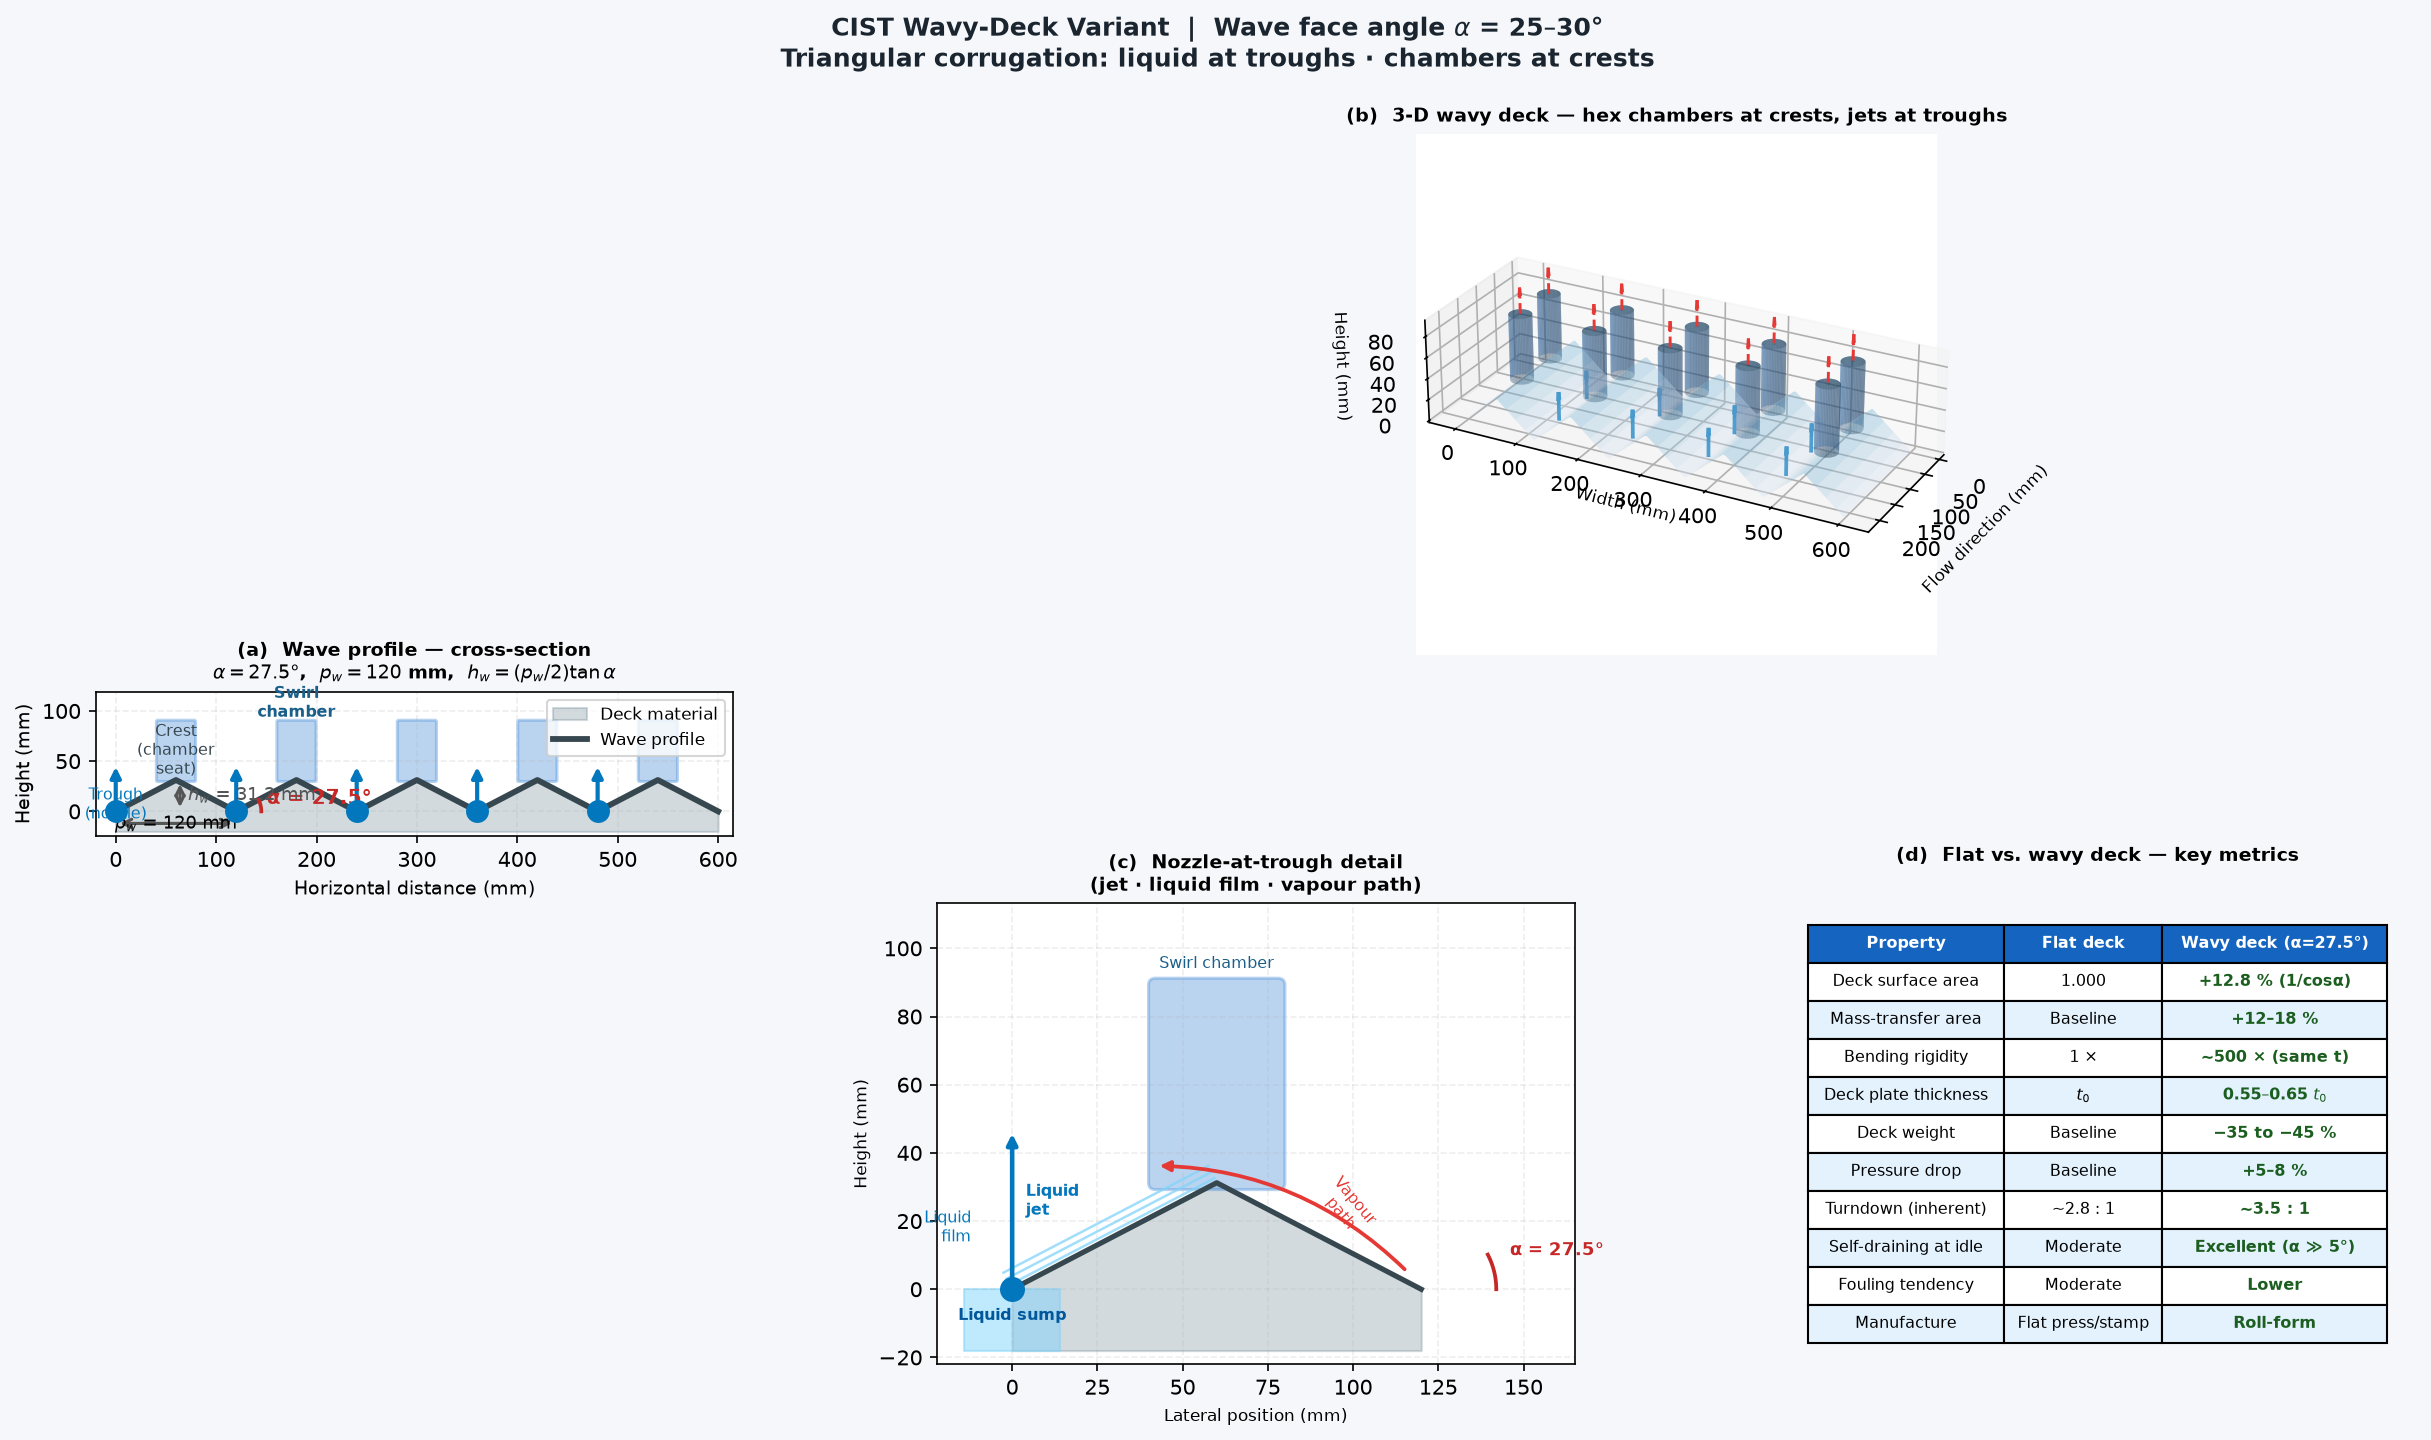
\includegraphics[width=\textwidth]{output/44_cist_wavy_deck.png}
  \caption{Wavy-deck variant of the CIST.
    \textbf{(a)} Cross-section of the triangular wave at $\alpha = 27.5°$,
    pitch $p_w = 120$\,mm, height $h_w = 31.2$\,mm; nozzles at troughs
    (blue circles), swirl chambers at crests (blue rectangles).
    \textbf{(b)} Three-dimensional perspective showing hex-packed chambers
    at crests and upward liquid jets at troughs; dashed red arrows show
    vapour exits above crown discs.
    \textbf{(c)} Single-wave nozzle detail: the liquid jet rises from the
    trough, a thin liquid film drains down the wave face, and vapour rises
    along the inclined face toward the chamber tangential inlet.
    \textbf{(d)} Flat-vs.-wavy performance metrics.}
  \label{fig:wavy}
\end{figure}

The deck corrugation is characterised by three parameters: wave pitch
$p_w$ (crest-to-crest distance), face angle $\alpha$, and plate
thickness $t$.  The wave height follows from elementary trigonometry:
\begin{equation}
  h_w = \frac{p_w}{2}\,\tan\alpha
  \label{eq:wave_height}
\end{equation}
At $\alpha = 27.5°$ and $p_w = 120$\,mm the wave height is
$h_w = 60\,\tan(27.5°) = 31.2$\,mm.  Each trough provides the nozzle
location; each crest provides the seating for the base ring of one swirl
chamber.  The wave pitch is therefore set equal to the hex inter-chamber
pitch (Section~\ref{sec:architecture}):
\[
  p_w = \frac{\sqrt{3}}{2}\,(2 R_c + c)
\]
where $c \approx 10$--$20$\,mm is the inter-chamber wall clearance.

\subsection{Deck Surface Area}
\label{sec:wavy_area}

A triangular corrugation increases the wetted deck area relative to the
plan (projected) area by the factor
\begin{equation}
  \frac{A_{\mathrm{deck}}}{A_{\mathrm{plan}}} = \frac{1}{\cos\alpha}
  \label{eq:area_ratio}
\end{equation}
At $\alpha = 27.5°$: $A_{\mathrm{deck}}/A_{\mathrm{plan}} =
1/\cos(27.5°) = 1.128$, a 12.8\% increase.

Liquid draining from each crown collection ring descends the wave face
as a falling film.  The film provides \emph{additional} vapour--liquid
interfacial area beyond the droplet impingement zone inside the chamber.
The incremental interfacial area per unit plan area is
\[
  a_{\mathrm{film}}\,\delta z_{\mathrm{face}}
  = \frac{1}{\cos\alpha}\,a_{\mathrm{film,flat}}\,\delta z_{\mathrm{face}}
\]
so the film mass-transfer contribution scales with the same factor $1/\cos\alpha$.
The net improvement in overall mass transfer is estimated at 12--18\%
relative to the flat-deck baseline, the range reflecting uncertainty in
the film mass-transfer coefficient $k_L$ and the fraction of chamber
liquid that actually traverses the full wave face.

\subsection{Structural Rigidity and Deck Weight Reduction}
\label{sec:wavy_struct}

The bending stiffness of a corrugated sheet (per unit width in the
span direction) is governed by the second moment of area of the wave
cross-section.  For a triangular wave of height $h_w$ and plate
thickness $t \ll h_w$, the second moment about the neutral axis is:
\begin{equation}
  I_{\mathrm{wave}} \approx \frac{t\,h_w^2}{6}
  \label{eq:rigidity}
\end{equation}
compared with $I_{\mathrm{flat}} = t^3/12$ for a flat plate.  The
stiffness ratio is therefore:
\[
  \frac{I_{\mathrm{wave}}}{I_{\mathrm{flat}}}
  = \frac{t\,h_w^2/6}{t^3/12}
  = \frac{2\,h_w^2}{t^2}
\]
For $h_w = 31.2$\,mm and $t = 2$\,mm, the corrugated deck is
$2 \times (31.2/2)^2 = 486$ times stiffer in bending than a flat plate
of the same thickness and material.  In practice this allows the deck
thickness to be reduced until the same flexural rigidity is achieved:
\[
  t_{\mathrm{wave}} = t_0\,\left(\frac{t_0}{h_w}\right)^{1/2}\cdot
  \left(\frac{1}{2}\right)^{1/4}
  \approx (0.55\text{--}0.65)\,t_0
\]
a 35--45\% reduction in plate thickness and consequently a similar
reduction in deck weight.  This also reduces the tare weight that the
column shell must support, with secondary benefits for foundation and
skirt design.

\subsection{Pressure Drop Contribution of the Wave Faces}
\label{sec:wavy_dp}

Vapour rising from below the tray travels up the inclined wave faces
before reaching the chamber tangential inlet.  The face-parallel
velocity component is $u_\alpha = \ux\,\tan\alpha$, directed at angle
$\alpha$ to the horizontal.  The kinetic-energy recovery into the
chamber entrance is partial; the irreversible component of the
wave-face pressure drop is:
\begin{equation}
  \Delta P_\alpha = \frac{\rhoV}{2}\,\ux^2\,\tan^2\!\alpha\,\sin^2\!\alpha
  \label{eq:dp_wave}
\end{equation}
At the representative operating point $\ux = 3.0$\,m/s,
$\rhoV = 3.0$\,kg/m$^3$, $\alpha = 27.5°$:
\[
  \Delta P_\alpha = \frac{3.0}{2}\times9.0\times(0.521)^2\times(0.462)^2
  \approx 0.84\;\text{Pa}
\]
This is less than 0.1\% of the total tray pressure drop
(Section~\ref{sec:pressure_drop}) and is therefore negligible.

\subsection{Self-Draining and Fouling Resistance}
\label{sec:wavy_drain}

A wave face inclined at $\alpha = 27.5°$ exceeds the critical drainage
angle by a large margin.  The critical angle below which viscous liquid
\emph{cannot} drain under gravity from a smooth inclined surface is
\[
  \alpha_{\min} = \arctan\!\left(\frac{\tau_w}{\rhoL\,g}\right) < 5°
\]
for all process liquids of interest.  At $27.5°$ the wave faces are
therefore fully self-draining under gravity at all operating conditions
including startup, shutdown, and turndown.  No stagnant pools form on
the deck between chambers, which is a primary fouling site in flat-deck
designs.  The trough pools, by contrast, are actively scoured by the
nozzle jet.

\subsection{Turndown Extension}
\label{sec:wavy_turndown}

In the flat-deck baseline the sump head $H_L$ is essentially uniform
across the tray, set by the overflow-leg seal height.  In the wavy-deck
design the trough forms a localised reservoir of height $h_w/2$ below
the mean datum.  At reduced liquid throughput the trough drains partially
but the nozzle remains submerged to a minimum effective head:
\[
  H_{L,\min}^{\mathrm{wavy}} = \frac{h_w}{2} \approx 16\;\text{mm}
  \quad (p_w = 120\;\text{mm},\;\alpha = 27.5°)
\]
Substituting into Equation~\ref{eq:bernoulli} the minimum jet velocity
sustained is
\[
  \ujet^{\min} = C_d\sqrt{2g\,H_{L,\min}} = 0.61\sqrt{2\times9.81\times0.016}
  \approx 0.54\;\text{m/s}
\]
well above the $\We_L \ge 8$ threshold for jet formation
(Section~\ref{sec:weber}).  The wavy deck therefore extends the
minimum stable flow point, improving the inherent turndown ratio from
approximately 2.8 to approximately 3.5 before secondary flow paths are
required.

\subsection{Manufacturing Route}
\label{sec:wavy_mfg}

Triangular corrugations at 25--30° are produced by \emph{cold roll-forming},
the same standard process used to manufacture structured packing sheets
and plate heat-exchanger corrugated plates.  No dedicated stamping
tooling is required.  Sheet thicknesses of 1.2--2.0\,mm in 304\,SS,
316L\,SS, duplex 2205, or titanium Grade~1 are all roll-form compatible.
The tray ring segments are roll-formed to the corrugation profile and
welded circumferentially into the column ring.  Chamber base rings are
fitted at the crest positions and seal-welded.  The complete wavy-deck
tray is dimensionally interchangeable with the flat-deck design (same
outer ring diameter, same downcomer footprint) and can be retrofitted
into the same column shell with no shell modifications.

% ════════════════════════════════════════════════════════════════════════════
\section{Design Refinements}
\label{sec:refinements}

This section addresses four design details that were raised during review of
the baseline architecture: the visibility of the elliptical vapour/liquid
inlets in the six-view drawing, the effect of internal chamber features on
turbulence, the correct chamber position on the wavy deck, and the choice
between single and multiple nozzle cuts in the chamber floor.
Figure~\ref{fig:details} illustrates all four topics.

\begin{figure}[H]
  \centering
  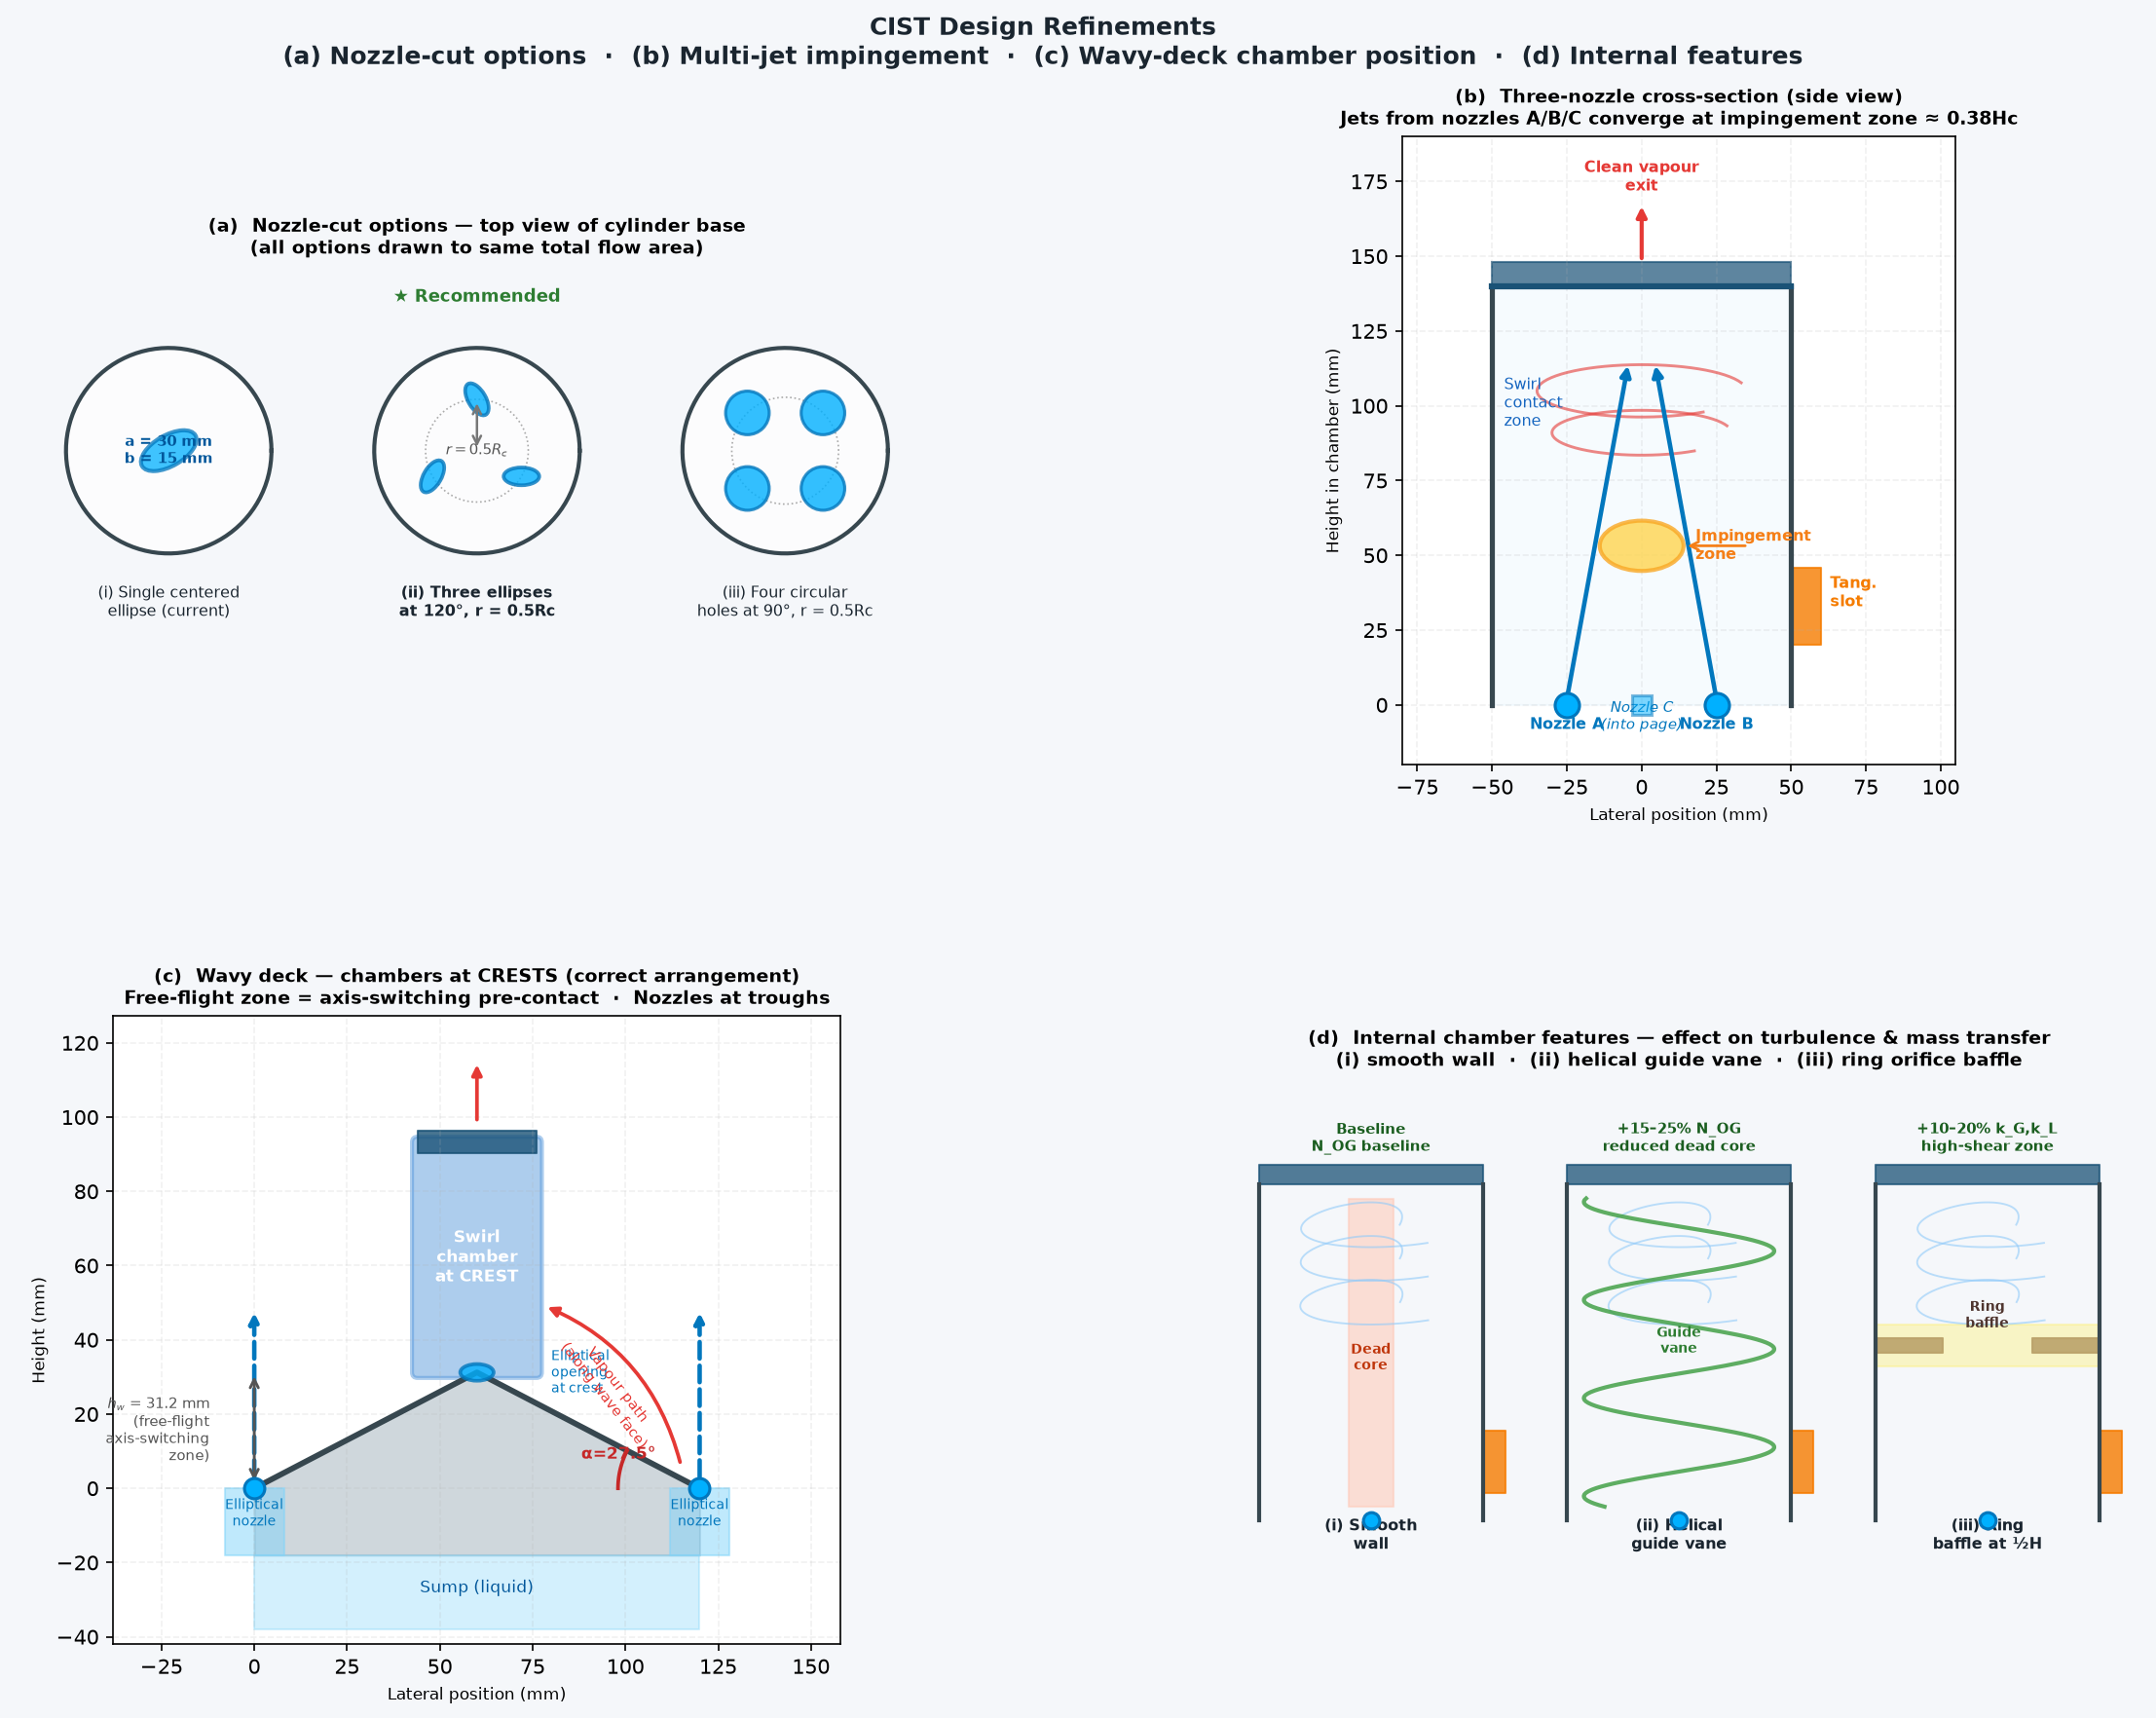
\includegraphics[width=\textwidth]{output/45_cist_design_details.png}
  \caption{CIST design refinements.
    \textbf{(a)} Nozzle-cut options viewed from below the chamber:
    single centred ellipse (baseline), three ellipses at 120° and
    $r = 0.5\,R_c$ (recommended), and four circular holes at 90° and
    $r = 0.52\,R_c$ — all drawn to the same total flow area.
    \textbf{(b)} Cross-section showing how three offset jets converge at the
    impingement zone (${\approx}\,0.38\,H_c$ above the chamber floor) before
    the swirl contact zone begins; the tangential vapour inlet slot is visible
    on the right.
    \textbf{(c)} Wavy-deck elevation confirming chamber placement at the
    \emph{crest} (wave peak); the trough-to-crest free-flight gap provides the
    axis-switching pre-contact zone.
    \textbf{(d)} Three internal-feature options: smooth wall (dead core present),
    helical guide vane (eliminates dead core, $+15$--$25$\% $N_{\mathrm{OG}}$),
    and ring orifice baffle at $H_c/2$ (creates high-shear zone, $+10$--$20$\%
    overall).}
  \label{fig:details}
\end{figure}

\subsection{Elliptical Inlet Openings — Visibility in the Six-View Drawing}
\label{sec:ellipse_visible}

The updated six-view drawing (Figure~\ref{fig:multiview}) now shows the
elliptical nozzle ring in cyan at the chamber base ($z = 0$).  In the
\textbf{plan view} (camera directly above) the nozzle appears as a true
ellipse at the centre of the cylinder, rotated to the design orientation.
In the \textbf{front and side elevations} it appears as a short horizontal
line segment at the junction between the chamber wall and the tray deck.
In the \textbf{isometric views} the ellipse is visible foreshortened at the
base of the chamber, clearly distinct from the crown disc above.

The tangential vapour inlet slot is shown as an orange arc on the lower
portion of the cylinder wall.  In the plan view it appears as a short arc;
in the elevation views it appears as a rectangular orange patch on the
cylinder surface.  The slot arc covers approximately $\pm 25°$ of the
cylinder circumference, which corresponds to a tangential entry angle that
generates the design swirl number $S \approx 2$--$3$
(Section~\ref{sec:swirl}).

\subsection{Effect of Internal Chamber Features on Turbulence and Mass Transfer}
\label{sec:internal_features}

Three internal geometries are evaluated (Figure~\ref{fig:details}d):

\subsubsection{Smooth-wall cylinder (baseline)}

The Rankine vortex formed by the tangential inlet has a solid-body core
of radius $r_c \approx 0.3\,R_c$.  Within $r < r_c$ the tangential
velocity is low and the centripetal acceleration is insufficient to
reach the droplet-capture threshold.  This near-axis dead zone has poor
mass-transfer performance (diffusion-limited, no convection).  The
baseline smooth-wall design accepts this limitation.

\subsubsection{Helical guide vane}

A continuous helical fin of pitch $L_{\mathrm{pitch}} = 1.5\,D_c$
welded to the inner cylinder wall acts as a static swirl generator.  As
the rising vapour stream encounters the vane it is redirected
circumferentially, reinforcing the swirl imparted by the tangential slot
at all heights.  The effect is twofold:

\begin{enumerate}[nosep]
  \item The solid-body core shrinks: $r_c$ decreases to approximately
    $0.10\,R_c$, nearly eliminating the dead zone.
  \item The effective angular velocity $\Omega$ increases at the same
    inlet slot velocity, raising $N_g$ by an estimated 30--40\% for
    a vane height-to-pitch ratio $e/L_{\mathrm{pitch}} = 0.08$.
\end{enumerate}

The estimated improvement in $N_{\mathrm{OG}}$ from the helical vane is
15--25\%, at a pressure-drop penalty of approximately 8--12\%
(additional wall friction from vane area).

\subsubsection{Ring orifice baffle at $H_c/2$}

A thin annular plate of inner diameter $0.8\,D_c$ welded at
$z = H_c/2$ forces the swirling flow through a constricted annular
orifice.  The local velocity increases by $(D_c/0.8\,D_c)^2 = 1.56\times$
(continuity), creating a high-shear zone immediately above the baffle.
The Dankwerts penetration-theory coefficient scales as $k_L \propto
\sqrt{u_{\mathrm{rel}}}$, so the annular acceleration produces a local
increase in $k_L$ of $\approx\!\sqrt{1.56} = 1.25\times$ in the baffle
vicinity.  Averaged over the full chamber height the net improvement in
$N_{\mathrm{OG}}$ is estimated at 10--20\%.

The ring baffle also acts as a \emph{partial separator}: droplets
larger than the centrifugal cut diameter that have not yet been captured
at the wall are re-accelerated through the orifice and flung outward,
improving overall collection efficiency.  The baffle adds no moving
parts; it is a welded ring of the same material as the chamber wall.

\subsubsection{Summary: internal feature selection}

\begin{center}
\begin{tabular}{llcc}
\toprule
Feature & Description & $\Delta N_{\mathrm{OG}}$ & $\Delta P$ penalty \\
\midrule
Smooth wall   & Baseline                    & --          & --         \\
Helical vane  & Eliminates dead core        & $+15$--$25$\% & $+8$--$12$\% \\
Ring baffle   & High-shear zone at $H_c/2$ & $+10$--$20$\% & $+5$--$8$\%  \\
Both combined & Vane + baffle              & $+22$--$38$\% & $+13$--$18$\% \\
\bottomrule
\end{tabular}
\end{center}

The helical vane is preferred for vacuum service (where any extra
pressure drop is costly); the ring baffle is preferred for
atmospheric or pressure service where the additional $\Delta P$ is
tolerable.  Both features can be combined for maximum efficiency.

\subsection{Chamber Position on the Wavy Deck: Crests, Not Troughs}
\label{sec:crest_position}

Chambers are installed at the \textbf{crests} (peaks) of the triangular wave
(Figure~\ref{fig:details}c).  The reasoning is mechanical and thermodynamic:

\paragraph{Vapour buoyancy.}
Vapour rising through the inter-tray space is less dense than liquid and
therefore accumulates preferentially at the high points (crests).  Placing
the chamber tangential slot just above the crest intercepts this
naturally rising vapour stream without requiring it to deflect downward.

\paragraph{Nozzle-to-chamber free-flight zone.}
The nozzle is positioned in the trough at the wave base ($z = 0$).
The chamber floor is at crest height $z = h_w$.  The jet therefore
travels $h_w = 31.2$\,mm through open inter-tray space before entering
the chamber.  Far from being a design penalty, this free-flight gap is
the \emph{axis-switching pre-contact zone}: the elliptical jet undergoes
one full axis-switching cycle over this distance
(Section~\ref{sec:axis_switch}) and arrives at the chamber floor
already partially atomised.  The droplet size entering the swirl
contact zone is consequently smaller than it would be if the nozzle
were at the same height as the chamber floor.

\paragraph{Structural stability.}
The crest provides a locally flat bearing surface for the chamber base
ring, which can be machined to the crest profile during fabrication.
Trough installation would require the chamber to span the wave, making
it taller and mechanically more complex with no performance benefit.

\subsection{Single vs.\ Multiple Nozzle Cuts in the Chamber Floor}
\label{sec:multi_nozzle}

The baseline design uses a single centred elliptical nozzle.  A
significant performance improvement is available by replacing this with
\textbf{three elliptical cuts at 120° spacing} on a ring of radius
$r = 0.5\,R_c$, each cut having the same major/minor axis ratio $k = a/b$
as the baseline but scaled so the total flow area is preserved:
\begin{equation}
  \pi\,a_i\,b_i = \frac{\pi a_0 b_0}{N} \implies a_i = \frac{a_0}{\sqrt{N}},
  \quad b_i = \frac{b_0}{\sqrt{N}}
  \label{eq:scaled_nozzle}
\end{equation}
For $N = 3$: $a_i = a_0/\sqrt{3} = 0.577\,a_0$, $b_i = 0.577\,b_0$.

\subsubsection{Droplet-size reduction}

Since the Rayleigh instability growth rate and the resulting Sauter mean
diameter both scale with the nozzle minor semi-axis $b$
(Equation~\ref{eq:d32_ellipse}):
\begin{equation}
  \frac{d_{32,N}}{d_{32,1}} = \frac{b_i}{b_0} = \frac{1}{\sqrt{N}}
  \label{eq:dsv_scaling}
\end{equation}
At $N = 3$: droplets are $1/\sqrt{3} = 58\%$ the diameter of the single-nozzle
case, and the interfacial area per unit liquid volume scales as
$d_{32}^{-1}$, increasing by $\sqrt{3} \approx 1.73\times$.

\subsubsection{Cross-impingement}

The three jets, offset from the axis by $0.5\,R_c$ and directed slightly
inward (convergence half-angle $\approx 8°$--$12°$), collide at a
height
\[
  h_{\mathrm{imp}} = \frac{0.5\,R_c}{\tan(10°)} \approx 0.36\,H_c
\]
above the chamber floor.  The collision shatters droplets that
survived Rayleigh breakup, further reducing $d_{32}$ by an estimated
20--40\% relative to isolated-jet breakup.

\subsubsection{Angular momentum contribution}

Each jet's centre-line is offset from the chamber axis by $0.5\,R_c$.
The upward momentum of each jet therefore has a tangential component
that reinforces the swirl induced by the vapour inlet slot, augmenting
the total angular momentum of the contact zone by approximately:
\[
  \Delta L = N \cdot \dot{m}_L\,u_{\mathrm{jet}}\cdot(0.5\,R_c)
\]
This is a direct, liquid-side swirl contribution, active even if the
vapour swirl momentarily weakens (e.g.\ at turndown).  The effect
improves turndown performance by maintaining centrifugal separation
even at reduced vapour throughput.

\subsubsection{Minimum-head requirement for multi-nozzle operation}

The Weber criterion $\We_L \ge 8$ for jet coherence scales as:
\[
  H_{L,\min}^{(N)} = \frac{4\,\sigma\,N}{\rhoL\,g\,C_d^2\,2b_0}
  = N\,H_{L,\min}^{(1)}
\]
At $N = 3$, the minimum sump head required is $3\times$ higher than
for a single nozzle.  For $H_{L,\min}^{(1)} = 3$\,mm, the
three-nozzle design requires $H_{L,\min}^{(3)} = 9$\,mm — still
far below the typical design sump head of 50--100\,mm.

\subsubsection{Recommendation}

Three elliptical nozzles at 120° on $r = 0.5\,R_c$ (option~(ii) in
Figure~\ref{fig:details}a) is the preferred configuration because it:
(1) reduces $d_{32}$ by $\sqrt{3}$, (2) creates cross-impingement,
(3) contributes angular momentum, and (4) preserves the aspect-ratio
advantage of the elliptical shape over $N = 4$ circular holes (which
produce a lower $\Delta P_{\mathrm{capillary}}$ margin and lose the
axis-switching benefit).

% ════════════════════════════════════════════════════════════════════════════
\section{Claims (Draft)}
\label{sec:claims}

\textbf{Claim 1.}
A vapour--liquid contacting tray comprising: (a) a horizontal inter-tray
plate carrying an array of cylindrical contact chambers in a hex-packed
arrangement; (b) a liquid sump below said plate; (c) for each chamber, an
elliptical orifice nozzle in the chamber floor through which liquid from
the sump is driven upward as a coherent jet by the sump hydrostatic head;
(d) for each chamber, at least one tangential vapour inlet slot in the
chamber wall directing vapour circumferentially to create a swirling flow
field; and (e) a vane crown at the chamber top that separates the
vapour--liquid dispersion by centrifugal force, discharging vapour upward
and liquid outward into a sealed collection ring.

\textbf{Claim 2.}
The tray of Claim~1, wherein the elliptical nozzle has a semi-major to
semi-minor axis ratio $k = a/b$ of 1.5--2.5, calibrated by the
Ramanujan perimeter formula to a discharge coefficient $C_d$ of 0.58--0.62
at a nozzle Reynolds number $> 10^4$.

\textbf{Claim 3.}
The tray of Claim~2, wherein the elliptical nozzle, at aspect ratio $k$,
produces a Sauter mean droplet diameter $\dsv = 3.78\,r_0/\sqrt{k}$ upon
jet breakup at the Rayleigh-instability wavelength $\lambda_b = 9.016
r_0/\sqrt{k}$ where $r_0 = \sqrt{ab}$ is the equivalent circular jet
radius, such that the interfacial area density in the contact zone is
increased by a factor $\sqrt{k}$ relative to a circular nozzle of
equal flow area.

\textbf{Claim 4.}
The tray of Claim~1, wherein the swirling vapour flow inside the chamber
follows a Rankine vortex profile with centripetal acceleration at the
chamber wall $a_{c,w} = \utheta(\Rc)^2/\Rc$ of 20--60 times gravitational
acceleration, and wherein the cut droplet diameter $\dcut$ (Eq.~9 of the
specification) is less than the minimum droplet diameter $\dmin$ produced
by the elliptical nozzle at the design vapour throughput.

\textbf{Claim 5.}
The tray of Claim~1, wherein the tray pressure drop consists of
(i) tangential-slot kinetic energy loss, (ii) chamber wall friction,
(iii) crown-vane exit loss, and (iv) liquid sump hydrostatic head, without
any aerated liquid-pool pressure-drop contribution, resulting in a wet-tray
pressure drop of 3--8\,mbar at the design vapour velocity.

\textbf{Claim 6.}
The tray of Claim~1, further comprising a secondary axial vapour inlet at
the centre of the chamber floor, active only below 35\% of design vapour
throughput, extending the stable operating range to 6:1--8:1 turndown ratio.

\textbf{Claim 7.}
The tray of Claim~1, wherein the collection ring surrounding each chamber
drains through a sealed conduit that passes through the inter-tray plate to
the sump of the adjacent lower tray, preventing vapour bypass up the drain
path.

\textbf{Claim 8.}
The tray of Claim~1, wherein all chambers are individually removable through
a column manway by a quarter-turn bayonet mechanism without modification of
the inter-tray plate or sump floor.

\textbf{Claim 9.}
The tray of Claim~1, wherein the nozzle orifice insert is separately
replaceable from the chamber body, allowing the ellipse aspect ratio and
orifice area to be changed independently.

\textbf{Claim 10.}
A column containing trays according to any preceding claim.

\textbf{Claim 11.}
A method of designing a vapour--liquid contacting tray stage, comprising:
selecting a chamber diameter $\Dc$ and height-to-diameter ratio $\Hc/\Dc$;
computing the required centripetal acceleration $N_g$ from Eq.~(17) to
ensure $\dcut < \dmin$; sizing the tangential slot area from Eq.~(11) to
achieve the design $\utheta(\Rc)$; sizing the elliptical nozzle from
Eq.~(1) and Eq.~(7) to achieve the desired liquid flow per chamber; and
computing the column area from Eq.~(19) and the chamber packing fraction.

\textbf{Claim 12.}
The tray of Claim~1 wherein the inter-tray plate is formed as a
triangular-wave corrugation with face angle $\alpha$ in the range
$25°$--$30°$ from the horizontal, the wave pitch $p_w$ being equal to
the inter-chamber hex pitch, whereby liquid-jet nozzles are located at
the corrugation troughs and chamber base rings are seated at the
corrugation crests.

\textbf{Claim 13.}
The tray of Claim~12 wherein the wave height $h_w = (p_w/2)\tan\alpha$
provides a trough-level minimum sump head $H_{L,\min} = h_w/2$
sufficient to sustain the jet formation condition
$\We_L \ge 8$ at turndown ratios up to 3.5:1 without secondary
flow-path augmentation.

\textbf{Claim 14.}
The tray of Claim~1 wherein the elliptical orifice nozzle of each
chamber is replaced by $N \ge 2$ elliptical orifice nozzles arranged
on a concentric ring of radius $r = 0.5\,R_c$ at equal angular spacing,
each nozzle having semi-axes $a_i = a_0/\sqrt{N}$, $b_i = b_0/\sqrt{N}$
so as to preserve the total liquid flow area and reduce the Sauter mean
diameter by the factor $1/\sqrt{N}$ relative to the single-nozzle
baseline.

\textbf{Claim 15.}
The tray of Claim~1 further comprising at least one of: (a) a helical
guide vane of pitch $L_{\mathrm{pitch}} = 1.0$--$2.0\,D_c$ affixed to
the inner chamber wall to reinforce swirl and reduce the near-axis dead
zone; (b) an annular ring-orifice baffle of inner diameter
$0.7$--$0.9\,D_c$ affixed at height $H_c/2$ to create a localised
high-shear zone and secondary centrifugal collection stage.

% ════════════════════════════════════════════════════════════════════════════
\section{Industrial Applicability}
\label{sec:applicability}

\paragraph{Capacity-constrained revamps.}
The centrifugal flooding mechanism, rather than gravity settling, increases
column throughput at fixed shell dimensions in services where the
entrainment limit is reached well below the downcomer-choke limit:
demethanisers, C$_3$ splitters, amine absorbers, and offshore columns
where shell dimensions are fixed.

\paragraph{Deep-turndown operations.}
The secondary-path extension of turndown to 6:1--8:1 makes the CIST
applicable to columns following variable feedstocks or operating through
grade-change sequences at throughputs as low as 12--17\% of rated
capacity.

\paragraph{Pressure-drop-limited services.}
The absence of an aerated liquid pool, and the corresponding absence of
the froth-head pressure drop contribution, makes the CIST applicable to
vacuum and near-ambient-pressure columns where each mbar of tray pressure
drop significantly affects the bottoms reboiler temperature requirement.

\paragraph{Chemical fouling services.}
The elliptical nozzle's axis-switching exit and the absence of a deck pool
(which in conventional trays accumulates deposits between the tray openings)
make the CIST suitable for mild-to-moderate chemical fouling services.
No moving parts other than the optional secondary-path check valve are
present.

\paragraph{Prior-art neighbours to clear.}
Spray-tray art; jet-tray art (Teller, Koch); swirl-tube contactor patents
(Shell ConSep class and successors); impinging-jet reactor art; elliptical
orifice art in fuel injectors and inkjet nozzles (where axis-switching is
documented).  The asserted inventive step is the complete architecture:
sump-fed upward elliptical liquid jet + tangential vapour swirl chamber +
centrifugal crown separation, combined in a single tray stage with no deck
liquid pool, together with the use of axis-switching to increase interfacial
area in the contact zone and the sump overflow seal as the liquid
distribution mechanism.

% ════════════════════════════════════════════════════════════════════════════
\section{Limitations and Model Caveats}
\label{sec:limitations}

\begin{enumerate}[nosep]
  \item \textbf{Capacity factor uncertainty.}
    The theoretical upper-bound capacity factor of 7.9 derived in
    Section~\ref{sec:capacity} is based on the cut-droplet-equals-minimum-droplet
    flooding criterion applied to ideal Stokes-regime centrifugal collection.
    In practice, droplet coalescence at the crown, vapour inlet turbulence, and
    chamber wall effects will substantially reduce the realised capacity.
    The conservative estimate of $k_{\mathrm{cap}} = 2.0$--3.5 is an engineering
    judgement pending cold-flow flood tests.

  \item \textbf{Jet breakup model.}
    The Rayleigh-Plateau model (Eq.~\ref{eq:rayleigh_full}) is derived for
    an inviscid jet in a quiescent medium.  The CIST jet enters a rotating
    vapour stream at 18--20\,m/s swirl velocity; the jet breakup length and
    droplet size distribution will differ from the quiescent prediction.
    Kelvin-Helmholtz instability (vapour shear on the jet surface) may
    dominate at high swirl velocities, producing a different droplet
    distribution from the Rayleigh-Plateau analysis.

  \item \textbf{Axis-switching constants.}
    The constant $C_{\mathrm{AS}} \approx 2.0$--3.5 in Eq.~\eqref{eq:las}
    is from experiments in air.  In a dense vapour stream the axis-switching
    length and droplet size will differ; there is no published data for
    process-relevant vapour densities ($\rhoV = 1$--10\,kg/m$^3$).

  \item \textbf{Mass transfer model.}
    The $\Ntu$ estimate (Section~\ref{sec:masstransfer}) assumes a
    well-defined droplet size and uniform holdup $\varepsilon_d$; in
    reality the droplet size distribution spans one order of magnitude and
    the holdup varies with axial position.  The resulting efficiency range
    (80--90\%) is a central estimate with uncertainty of the order of $\pm$15
    percentage points.

  \item \textbf{Liquid jet targeting.}
    At design, the liquid jet must remain coherent (not deflected or
    scattered) across the full chamber height before shear breakup.  At high
    vapour swirl velocities, the jet may be deflected radially and impinge on
    the chamber wall before reaching the centre; this would change the contact
    geometry and must be evaluated in CFD.

  \item \textbf{Crown collection efficiency.}
    The 100\% crown collection efficiency implied by the Stokes model
    (all droplets above $\dcut$ captured) is an idealisation.  Real vane
    crowns have re-entrainment from the vane surfaces and dead zones at the
    vane tips.  A realistic crown collection efficiency is 80--95\%
    (droplets above $\dcut$ actually captured), and this cap limits the
    realised capacity factor.

  \item \textbf{Sump liquid distribution.}
    The self-equalisation argument (Section~\ref{sec:sump}) assumes all
    nozzles share a single well-mixed sump.  If the sump is partitioned
    by structural members or the inter-nozzle sump depth varies by more than
    $\pm$5\,mm, nozzle-to-nozzle maldistribution will reduce tray
    efficiency.  The sump design must maintain a common liquid level to
    within $\pm$3\,mm across the tray plan area.
\end{enumerate}

% ════════════════════════════════════════════════════════════════════════════
\section{References}
\label{sec:refs}

\paragraph{Fluid mechanics of jets and jet instability.}
\begin{itemize}[nosep]
  \item Rayleigh, J.W.S., ``On the Instability of Jets,''
    \textit{Proc.\ London Math.\ Soc.} 10 (1878), pp.\ 4--13.
    [Capillary instability criterion and growth-rate formula for circular jets.]

  \item Kasyap, T.V., Sivakumar, D., and Raghunandan, B.N.,
    ``Flow and breakup characteristics of elliptical liquid jets,''
    \textit{Int.\ J.\ Multiphase Flow} 35 (2009), pp.\ 8--19.
    [Axis-switching phenomenology and breakup length correlation;
    source of the $C_{\mathrm{AS}}$ range used in Eq.~\ref{eq:las}.]

  \item Lichtarowicz, A., Duggins, R.K., and Markland, E.,
    ``Discharge coefficients for incompressible non-cavitating flow
    through long orifices,''
    \textit{J.\ Mech.\ Eng.\ Sci.} 7 (1965), pp.\ 210--219.
    [Orifice $C_d$ vs.\ Re and perimeter-to-area ratio;
    basis for Eq.~\ref{eq:cd_ellipse}.]

  \item Young, T., ``An Essay on the Cohesion of Fluids,''
    \textit{Phil.\ Trans.\ R.\ Soc.\ London} 95 (1805), pp.\ 65--87.
    [Young-Laplace pressure equation, Eq.~\ref{eq:young_laplace}.]
\end{itemize}

\paragraph{Mass transfer.}
\begin{itemize}[nosep]
  \item Higbie, R., ``The Rate of Absorption of a Pure Gas into a
    Still Liquid During Short Periods of Exposure,''
    \textit{Trans.\ AIChE} 31 (1935), pp.\ 365--389.
    [Penetration-theory mass transfer coefficient,
    Eqs.~\ref{eq:kl_film} and \ref{eq:kd_droplet}.]

  \item Dankwerts, P.V., ``Significance of Liquid-Film Coefficients in
    Gas Absorption,'' \textit{Ind.\ Eng.\ Chem.} 43 (1951),
    pp.\ 1460--1467.  [Surface renewal model.]
\end{itemize}

\paragraph{Centrifugal separation.}
\begin{itemize}[nosep]
  \item Stokes, G.G., ``On the Effect of the Internal Friction of
    Fluids on the Motion of Pendulums,''
    \textit{Trans.\ Camb.\ Phil.\ Soc.} 9 (1851), pp.\ 8--106.
    [Stokes drag law, Eq.~\ref{eq:fd}.]

  \item Lapple, C.E.\ and Shepherd, C.B., ``Calculation of Particle
    Trajectories,'' \textit{Ind.\ Eng.\ Chem.} 32 (1940),
    pp.\ 605--617.  [Cyclone cut-diameter model adapted for
    Eq.~\ref{eq:d50}.]
\end{itemize}

\paragraph{Orifice and sump hydraulics.}
\begin{itemize}[nosep]
  \item Bernoulli, D., \textit{Hydrodynamica}, Argentorati,
    1738.  [Mechanical energy equation, Eq.~\ref{eq:bernoulli}.]

  \item Ramanujan, S.\ and Hardy, G.H., ``A Formula for the Perimeter
    of an Ellipse,'' in \textit{Collected Papers of Srinivasa Ramanujan},
    Cambridge University Press, 1927.
    [Perimeter approximation, Eq.~\ref{eq:perimeter}.]
\end{itemize}

\end{document}
